\documentclass[a4paper,english]{article}
\usepackage{graphicx}
\usepackage{fourier} %font
%\usepackage{lmodern} %default font
\usepackage[T1]{fontenc}
\usepackage[utf8]{inputenc}
\usepackage{babel}
\usepackage{hyperref}
\usepackage{upgreek} %proper greek letters
\usepackage{fullpage}
\usepackage{lineno}
\usepackage{amsmath} % typesetting math
\usepackage{amssymb}
\usepackage{booktabs} % nice tables
\usepackage[round,sort&compress]{natbib}
\usepackage{pdfpages} %include external pdfs
\usepackage{color} %colorcoding for remarks
\usepackage{enumitem} %for noitemsep in lists
\usepackage{subfig}
\newcommand\ds[1]{\color{red}#1\color{black}}
\newcommand\et[1]{\color{blue}#1\color{black}}
\newcommand\bh[1]{\color{green}#1\color{black}}
\renewcommand{\arraystretch}{1.2} % space in tables
%\usepackage{amsaddr}
\usepackage{authblk}
\usepackage[titletoc,title]{appendix} %for appendix titles

\begin{document}

%\title{Fall-off position estimation with collimated Prompt Gamma cameras in clinical simulations}
%\title{Spot grouping demonstrated with collimated Prompt Gamma cameras in clinical simulations}
\title{Performance of Prompt Gamma fall-off detection in clinical simulations}

\author[1,2]{Brent F. B. Huisman}
\author[2]{É. Testa}
\author[1]{D. Sarrut}
\affil[1]{~CREATIS, Université de Lyon; CNRS UMR5220; INSERM U1206; INSA-Lyon; Université Lyon 1; Centre Léon Bérard, Lyon, France}
\affil[2]{~IPNL, Université de Lyon; CNRS/IN2P3 UMR5822; Université Lyon 1 Lyon, France}
\affil[ ]{~E-mail: mail@brenthuisman.net}

\maketitle

\begin{abstract}

\emph{Purpose:} There is interest in the particle therapy community to use Prompt Gammas (PG) for treatment verification and eventually dose control. As the first detectors are deployed in clinical setting, we present a feasibility study of PG fall-off position (FOP) estimation using PG cameras with active beam delivery; the first where CT, treatment plan (TP) and beam description are all clinical data. Firstly, we investigate TP spot weight compositions, to establish what typical clinical spot weights are. Then, the statistics required for a consistent FOP estimate is investigated for two PG detectors. Finally, a spot-grouping method is proposed that combines better measurement statistics with fall-off preservation.

\emph{Materials and Methods:} Our starting point is a study of spot weight distributions, based on TPs provided by various proton clinics in Europe. A head and neck case with a CT and replanning (RP)CT was selected for the PG detection study. A proton TP was constructed on the CT according to clinical protocols and irradiated in silico on both CT and RPCT. During the irradiation, two PG cameras implemented according to their published specifications, a multi-parallel-slit (MPS) and knife-edge (KES) camera, recorded the PG profile. A simple FOP estimation algorithm is presented, and executed on 20 CT and 20 RPCT realizations to obtain a shift distribution. A selected spot has its weight modulated, in order to study shift distributions as function of the spot weight, for each camera. Then, an iso-depth ion-range based spot-grouping method is presented and compared to iso-energy spot-grouping.

\emph{Results:} Three spots were selected for an in depth study, and at the prescribed spot weights were found to produce results of insufficient precision, rendering usable clinical output on the spot level unlikely. When the spot weight is artificially increased to $10^9$ primaries, the precision on the FOP reaches millimetric precision. On the FOP shift the MPS camera provides between 0.77 - 1.15 mm (1$\upsigma$) precision for the three spots at $10^9$ protons; the KES between 1.93 - 2.25 mm.

\emph{Conclusion:} 

While with spot measurements the measured shift was in agreement with the PG emissions shift, for both grouping methods this was not the case, unless the emissions was convolved with a point spread function to estimate the detected signal. The precision on the shift obtained with iso-depth grouping improved significantly with respect to iso-energy grouping for the KES camera (1$\upsigma$ = 3.82 and 2.87 mm, iso-energy and iso-depth resp.), but not significantly for the MPS (1$\upsigma$ = 1.17 and 1.05 mm, iso-energy and iso-depth resp.). It is shown that grouping spots does not necessarily negatively affect the precision compared to the artificially increased spot, which means some form of spot grouping can enable clinical use of these PG cameras, if the sum of the spot weights is at least $10^9$ proton primaries. With all spots or spot groups the MPS has a better signal compared to the KES, thanks to a larger detection efficiency and a lower background level due to time of flight selection.

\end{abstract}


%%%%%%%%%%%%%%%%%%%%%%%%%%%%%%%%%%%%%%%%%%%%%%%%%%%%%%%%%%%%%%%%%%%%%%%
\section{Introduction}

The well-defined range of particles in matter is the main reason they are used in cancer treatment today. Unfortunately we are not able to take full advantage of this property, because of uncertainties in patient positioning, uncertainties on the proton range due to unknown displacements or deformations of organs, ill-defined lung, bowel or bladder filling, weight loss, and the inherent uncertainty in the Hounsfield unit to particle stopping power conversion \citep{Paganetti2013}. Often, medical practice is to plan conservatively, namely adding margins around the tumor, greatly reducing the potential benefits of particle treatment \citep{Knopf2013}. For example, irradiation fields with organs at risk (AOR) located just behind the Bragg Peak (BP) position are usually avoided, although they would better spare the AOR. Some form of in-vivo, online monitoring is generally considered to be a way out of this predicament. Online monitoring would make measurements of uncertainties such as mentioned above possible, and thereby permit more precise planning which could take maximum advantage of the steep BP fall-off and reduce damage to tissues surrounding the tumor.

Currently treatments can be verified by way of (offline) PET \citep{Kraan2015}. Integrating PET imaging in the beam gantry to reduce the effect of washout is being investigated \citep{Sportelli2013}. Another way to perform monitoring is to use prompt gammas (PGs), a natural byproduct in particle treatments. PGs offer the potential of monitoring treatment at the spot level \citep{Smeets2012,Roellinghoff2014a} and are therefore of prime interest \citep{Moteabbed2011,Gueth2013,Golnik2014a,Janssen2014}. These particles are produced in the inelastic nuclear collisions between the incident particle and the medium (tissue) it is traveling through, and they correlate strongly with dose deposition. This has been experimentally demonstrated for protons by \citet{Min2006} and for carbon by \citet{Testa2008}. A knife-edge PG camera \citep{Perali2014,Richter2016} was put into clinical operation in fall 2015, at OncoRay in Dresden, Germany. The aim of such collimated cameras is to obtain a 1D profile of the PG production along the beam direction and obtain the position of the fall-off of the signal, which is strongly correlated to the BP position. Other approaches include detection of the target materials using a spectral PG camera \citep{Verburg2014}, using the primary particle's time of flight (ToF) in a timed PG measurement \citep{Golnik2014a} and Compton camera designs \citep{Roellinghoff2011,Kurosawa2012,Solevi2016,Thirolf2016,Polf2015,Llosa2016}.

Here we present an in silico study of the clinical relevance of fall-off position (FOP) estimation, based on two collimated PG camera designs: a multi-parallel-slit (MPS) and knife-edge (KES) design. First, we start with an analysis of the composition of clinical treatment plans (TPs). The main determinant for the available PG signal is the number of primary protons per quantity of interest (whole treatment, iso-energy layer, spot or otherwise). Depending on target type, location, and size the spot distribution varies. That is to say: the number of spots, their average number of protons and their energy distribution have consequences for PG detection. Then, a brief analysis of the data and some treatment planning effects are presented in context of these spot distributions. In the second part of this paper, performances of the two PG cameras are studied on a clinical case, fully implemented in Gate. For a patient with a cranial tumor, significant weight loss was observed and a replanning CT (RPCT) obtained. The planning and replanning CTs provide an excellent 'easy' case where PG camera should reliably detect the difference. We begin with a study of the minimum number of protons required for a reliable FOP retrieval. To conclude, we propose two spot-grouping methods that improve the reliability of fall-off retrieval. %10 realizations per spot (per number of primaries) are created with the CT and RPCT, and thus 100 possible fall-off shifts are obtained.% The implications for the future of PG detection is discussed, and a method for spot summing is proposed.

%%%%%%%%%%%%%%%%%%%%%%%%%%%%%%%%%%%%%%%%%%%%%%%%%%%%%%%%%%%%%%%%%%%%%%%
\section{Materials and Methods}

\subsection{Preliminary observations / Clinical Analysis}

PG literature often quotes $10^8$ protons as the reference number of primaries per spot in proton therapy. Precision estimates are therefore usually obtained for statistics of this order, although higher spot intensities are not uncommon, even in phantom studies \citep{Priegnitz2016}. Spot-by-spot (range) verification with one or two millimeter fall-off retrieval precision would be the eventual result, which is very appealing. We conducted a small study into the spot weight prescribed by current treatment planning software (TPS) to help focus the targets that PG cameras must be able to reach. Apart from detector performance and PG discrimination, the main determinant of the PG signal is, after all, the spot weight.

\subsubsection{Treatment plan analysis}\label{sec:tpanalysis}

In \cite{Smeets2012} the composition of a particular TP is displayed: a scatter plot of the spot intensity as function of the proton energy. In greyscale the $1\upsigma$ precision on the fall-off retrieval with the IBA Knife-Edge PG camera prototype, at that time, is colored in. Only for the spots with the highest intensities is the precision lower than 2 mm. Our Elekta Xio TPS produces similar maximum spot intensities. Our TPs are created for an IBA proton accelerator with scanning nozzle \citep{Grevillot2011}, which have some spots with $10^8$ primaries at their top ends. More modern accelerator designs are able to produce smaller spots, more closely packed, in order to increase dose conformity. Alternatively, moving the patient closer to the beam nozzle, non-isocentric planning, is a recent development \cite{Grevillot2015} enabling smaller spots. TPS uses the higher number of spots to produce more conformal TPs, at the 'cost' of a lower average spot-intensities. Our TPS produces plans with about 500 to 1000 spots per field, while newer accelerators and associated plans may have thousands of spots per field (see figure~\ref{fig:planhigh}).

We analyzed a small set of clinical TPs to establish what clinical spot counts and proton counts per spot (spot weights) are, of which we present three 'archetypes' obtained from Uppsala University Hospital: a low precision case, a typical, medium precision case and a high precision case.

\begin{enumerate}[noitemsep]
\item Low precision: Arteriovenous Malformation (AVM) case, figure~\ref{fig:planlow}.

\begin{figure}[htp]
  \centering
  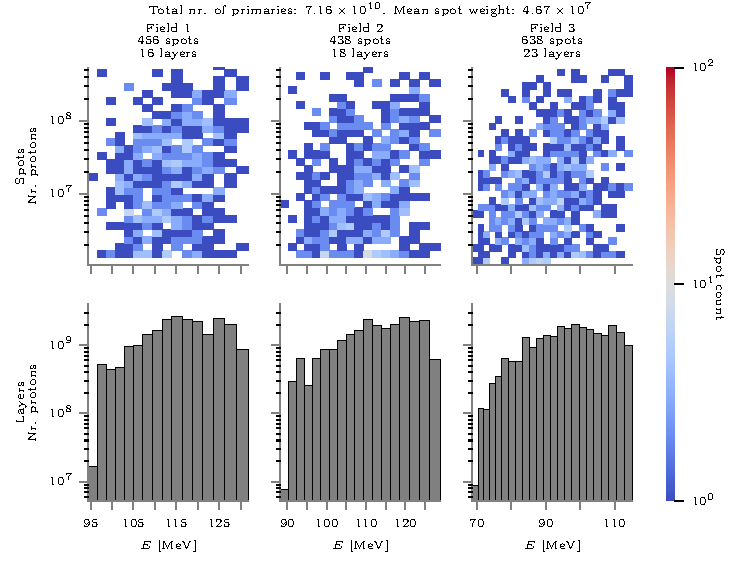
\includegraphics[width=0.8\linewidth]{AVM_F1nonorm-plot}
  \caption{TP for a Arteriovenous Malformation (AVM) case, provided by Erik Almhagen and created in the Uppsala University Hospital, Sweden. On top: the spots are binned as function of energy and spot weight (number of protons), with high spot counts in red (hot spots) and low spot counts in blue (cool spots).}
  \label{fig:planlow}
\end{figure}

\item[] AVMs are not cancers, but tangles of blood vessels that divert arterial blood from the brain. The dose tolerance is high (up to 10\%) in such cases. This high tolerance leads to fewer spots, with on average a higher proton count, which enables a quicker TP delivery and therefore higher patient throughput.% While the high proton count per spot seems in favor of PG monitoring, the high dose tolerance indicates little clinical interest.

\item Typical precision: Meningioma case, figure~\ref{fig:planmid}.

\begin{figure}[htp]
  \centering
  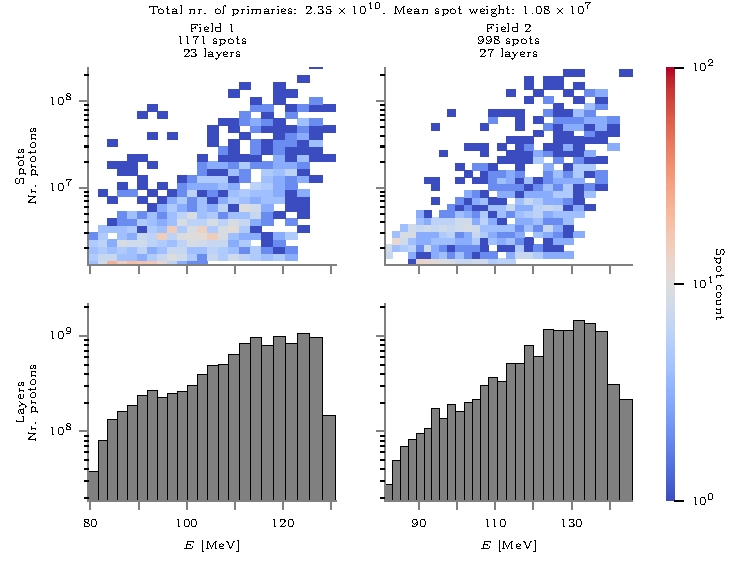
\includegraphics[width=0.8\linewidth]{MENINGIOMA_F1nonorm-plot}
  \caption{TP for a Meningioma case, provided by Erik Almhagen and created in the Uppsala University Hospital, Sweden.}
  \label{fig:planmid}
\end{figure}

\item[] Cases such as these are common in Uppsala University Hospital. These medium tolerance plans involve a lower average proton count per spot with respect to the AVM case. Some spots reach the type of statistics that is commonly quoted in PG literature. This being a good representation for typical plans insofar we have been able to establish, it would be correct to uphold $10^8$ protons as typical \emph{for the maximum weight spots}. As presented in the figure, the mean spot-weight here is $1.08\cdot10^7$.

\item High precision: a large and complex pediatric brain and spine case, figure~\ref{fig:planhigh}.

\begin{figure}[htp]
  \centering
  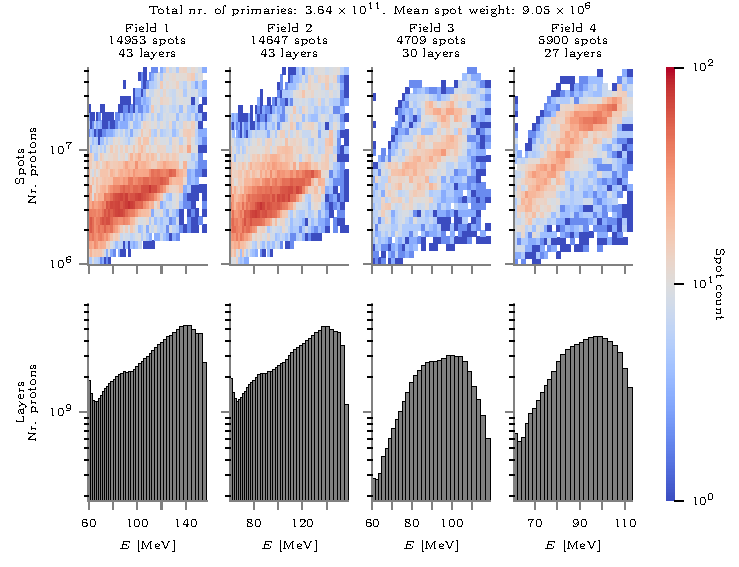
\includegraphics[width=0.8\linewidth]{CSI_F1nonorm-plot}
  \caption{TP for a large and complex pediatric brain and spine case. The left two fields are for the brain, the right two for the spine.}
  \label{fig:planhigh}
\end{figure}

\item[] Smaller spots, and therefore more spots, are used in plans where dose conformality is more pertinent. Much lower tolerances than usual are set because the patients are young and the side-effects must be minimized, which explains why the spot-count is over an order of magnitude more than the other TPs. This increase is accompanied with a decrease in per spot proton counts. The mean spot weight does not exceed $10^7$, with the majority of spots below this number.
\end{enumerate}

In conclusion, the number of spots can vary over more than an order of magnitude per plan, and therefore spot intensities inversely vary over an order of magnitude as well. The trend most plans follow is roughly an oval spot distribution, tilted towards a positive correlation with energy. Translated to energy layers, the intensities roughly follow a forwardly skewed normal distribution. The negative correlation between the typical spot weight and plan robustness is an important observation, and presents a challenge: in robust plans where precision is required, and treatment verification seems most pertinent, PG cameras must be able to deal with lower spot weights than previously anticipated. %Since the interest of treatment monitoring is most pertinent to such sensitive and complicated cases, we interpret this plot as a significant challenge for the PG community if per-spot monitoring is ever realized.

\subsubsection{Iso-energy layers vs. iso-depth layers}\label{sec:layers}

An evolved version of the IBA Knife-Edge PG camera has been put into clinical testing at OncoRay, Dresden \citep{Richter2016}. Because at the moment of the test, this facility had passive beam shaping, PG imaging could only take place on the iso-energy layer level. Apart from the most distal and proximal layers, per-layer weights are close to or over over $10^9$ primaries. This can be explained by the fact that tumor shapes are typically globulous, which means the most deeply penetrating energies only have to cover a small part of the transverse field (fig.~\ref{fig:planning}). Depending on the entrance position, the tumor shape and any (large) density deviations in the beam paths, an iso-energy layer in general does not correspond to a iso-depth layer. However, a collimated PG camera measures the PG yield as function of position along the beam axis; it measures PG yields per iso-depth layer. Collected counts per iso-energy layer then implies range mixing.

\begin{figure}[htp]
  \centering
  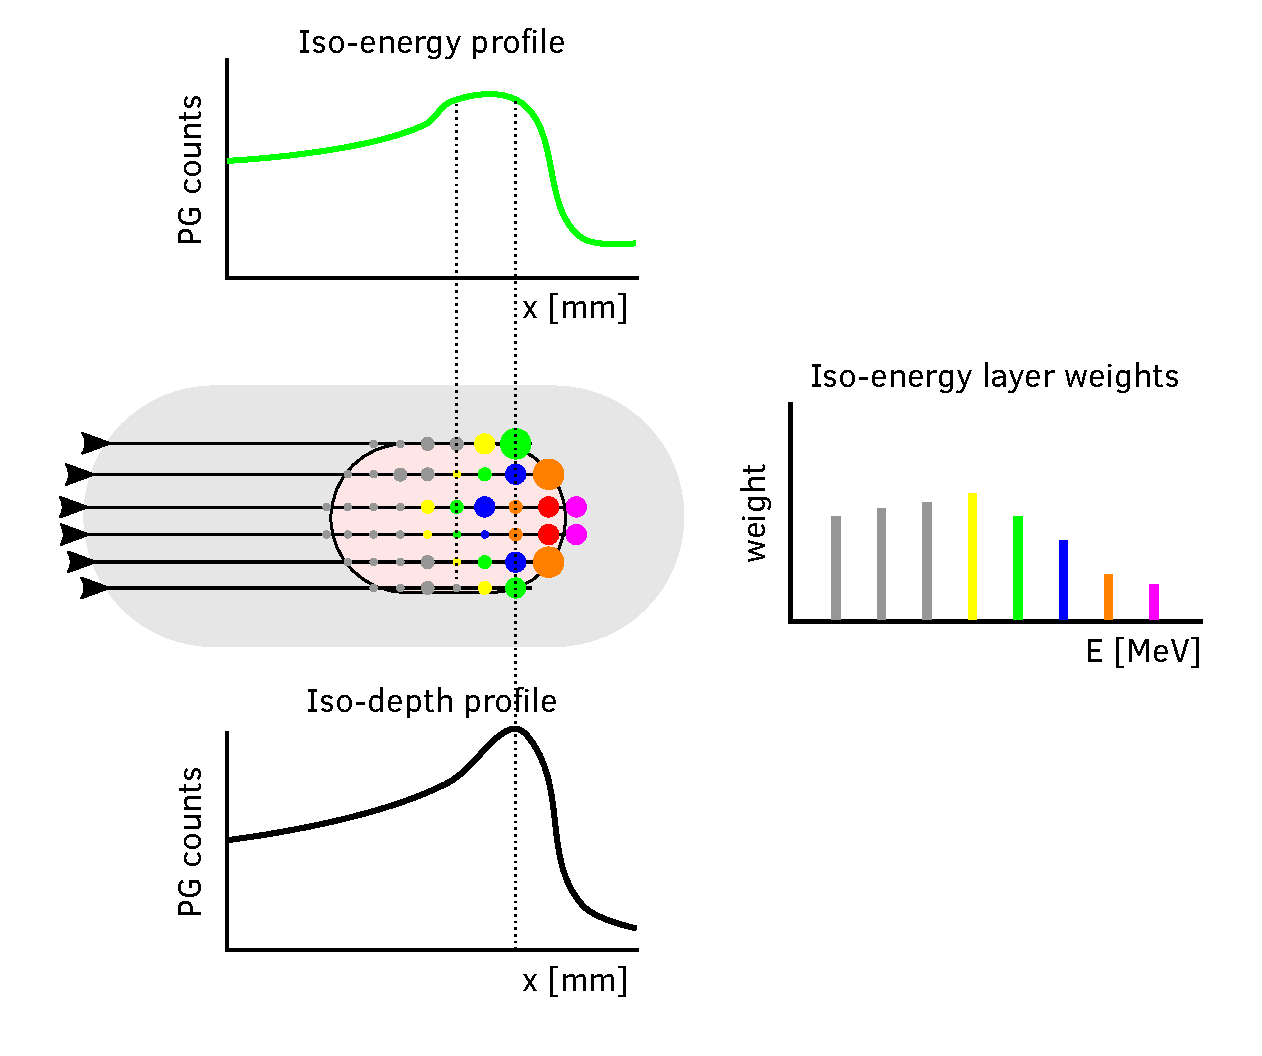
\includegraphics[width=0.6\linewidth]{planning}
  \caption{A schematic view of a patient (light gray), planned treatment volume (peach-pink), and a proton beam (black horizontal lines coming in from the left). Superimposed are various spots, where the size of the circles indicate spot weights. The spot colors indicate the iso-energy layer of which the spot is part. On the right, the weights (proton counts) per iso-energy layer are plotted, in similar fashion to fig.~\ref{fig:planmid}. On top, the PG profile is sketched for an iso-energy layer. On the bottom, the PG profile is sketched for iso-depth layer (spots of various color on the dotted line). In violet and red, the four dots on the distal end of the two most central beam lines, the effect of interpolation is illustrated: not always is every distal spot planned with a high weight.}
  \label{fig:planning}
\end{figure}

In particle therapy and particle therapy imaging literature we often see it mentioned that a spread out Bragg Peak (SOBP) is achieved by giving the most distal iso-energy layer the highest weight and each successive iso-energy layer is of lower energy and of lower weight. This is correct on the spot-level, for homogeneous phantoms, and when interpolation is not required. Interpolation happens when the energy levels of the beam delivery system do not correspond with the distal tumor contour \citep{0031-9155-57-21-N405}, in which case the dose contour is approximated by spreading the distal dose of the nearest two possible energies. In general, for clinical cases, the correlation between energy and range is only true in a general sense, as supported by the vertical spread in fig.~\ref{fig:planmid}. The maximum weight spots are often seen one of the most distal energy layers but not necessarily in the most one. Moreover, the weights of the distal layers are rarely the highest, so the accepted wisdom of the distal iso-energy layer being the most intense and thus most pertinent to range verification, must be challenged.

%The interest of PG detection is gathering data about the delivered dose in real-time. Whole-plan or partial-plan verification is a good start and such results have been published \cite{Richter2016}. However, as mentioned in the introduction, the most promising use of PG detection would be to track on the spot-level. To cope with low yields, it might be considered to group spots (in geometrical proximity for instance) or on the iso-energy layer level.

%In particle therapy and particle therapy imaging literature we often see it mentioned that a spread out Bragg Peak (SOBP) is achieved by giving the most distal iso-energy layer the highest intensity and each successive iso-energy layer is of lower energy and of lower intensity. This view makes sense for PTVs with a rectangular shape and rectangular targets, but of course patients do not fit that model. The surface where the beam impinges the patient is, seen perpendicular to the beam path, not flat, but curved, as is the entrance and exit surfaces of the PTV. This leads to the effect that the geometrically distal layer requires various energies (iso-energy layers), see fig.~\ref{fig:planning}. In other words, energy-layers alone are not a suitable proxy for geometrical position, and therefore not for range verification. It is important to separate iso-depth layers and iso-energy layers.

\subsection{PG camera modeling}\label{sec:camera}

%\subsubsection{Two Detectors}

As PG detectors we chose two prototypes that are tailored to FOP verification (illustrated in fig.~\ref{fig:detectors}):
\begin{itemize}[noitemsep]
\item the CLaRyS multi-parallel-slit (MPS) camera, Case 1 \citep{Pinto2014a}
\item[] The paper describes the optimization study of a multislit camera, where parameters such as collimator pitch, axis-to-collimator and axis-to-detector were varied, and their impacts evaluated on three criteria: 
\begin{itemize}[noitemsep]
\item Case 1: best precision on the FOP
\item Case 2: best precision on the profile length
\item Case 3: best precision on the FOP with a FoV lower than 15 mm
\end{itemize}
Each criterion resulted in a different optimal configuration. We are interested in the fall-off retrieval performance, which is why we select Case 1. As was done by \cite{Pinto2014a}, the lengths are chosen \emph{up to} 300 mm, such that the length is an integer multiple of the pitch size, with for the collimator a collimator-leaf-width extra, to ensure each pixel has a leaf on both sides. With the 8 mm pitch and 2.6 mm collimator-leafs, this results in a scintillator volume of length 296 mm and collimator length 298.6 mm.
%We note that \cite{Pinto2014a} describes a BGO absorber of 250 mm length along the beam axis, but present PG profile plots with data for 300 mm (figure 9). The collimator is about 300 mm along the beam direction, and it would have been natural for a multislit design to match these dimensions. We therefore will consider an absorber of 300 mm length as well. Our second note is that,
\item the IBA knife-edge (KES) camera \citep{Perali2014,Sterpin2015}
\item[] The IBA knife-edge camera has seen the first clinical test of a PG camera. \cite{Richter2016} provides the first clinically obtained results. At this time, no other camera has been subjected to clinical tests, which is why we consider this prototype a benchmark.
\end{itemize}

\begin{figure}[htp]
  \centering
  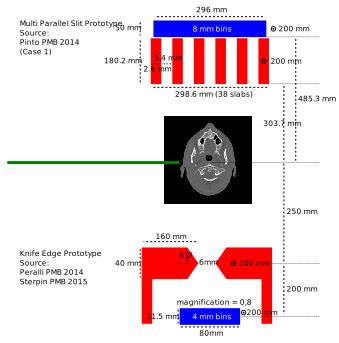
\includegraphics[width=0.9\linewidth]{detectors}
  \caption{Schematic presentation of the two PG cameras considered in this study. The green arrow represents the proton beam. In red the collimation elements and in blue detection elements. The dimensions were taken from \cite{Pinto2014a} and \cite{Perali2014,Sterpin2015}. Note that the two cameras were positioned at an identical location above the head during all simulations.}
  \label{fig:detectors}{fig:detectors}
\end{figure}

An important detail is the fact that \cite{Pinto2014a} carried out the optimization with a ToF selection window. Such a selection removes part of the background, based on the fact that the PG production is pulsed synchronous to the beam, while neutron-induced background is delayed. For the IBA C230 accelerator with a period of 10 ns, \cite{Pinto2014a} chose a window of 4 ns around the PG maximum, based on experimental ToF spectra. This means that about 60\% of the noise could be removed. For the KES prototype ToF is not used, leading to a higher background, as is evident when one compares the backgrounds as published in the two publications. A second difference is the energy selection window. The IBA group employ a 3-6 MeV window, whereas the CLaRyS collaboration produced their optimization with a 1-8 MeV window. We will compare each camera with their published properties, that is to say: a 1-8 MeV window and ToF for MPS and a 3-6 MeV window without ToF for KES.

% We will however also compare the cameras under similar circumstances. if we re-add ToF and energycut analysis

\subsection{Simulation}

Imaging paradigms such as PG detection are validated against experiments, and often also with Monte Carlo (MC) simulations~\citep{Moteabbed2011,Gueth2013,Robert2013,Golnik2014a,Janssen2014}. For rarely occurring processes such as PG simulation, convergence to the model of the truth to within acceptable statistical error can be slow. This paper presents an in silico study of the feasibility of the clinical relevance of PG FOP estimation using collimated cameras (section~\ref{sec:camera}), and uses the vpgTLE variance reduction method described in \cite{Huisman2016}. In brief, a full \emph{voxelized Prompt-Gamma Track Length Estimator} (vpgTLE) simulation is broken up into two stages. In stage one, a PG yield distribution image (PGyd) is created, specific to a particular phantom (or CT-image) and primary source (e.g. a treatment plan, a single spot). This PGyd image stores, per voxel per PG energy bin, the yield per primary. Stage two uses the PGyd and the assumption of isotropic PG emittance to generate and propagate the PGs throughout the rest of the geometry that the user has defined (e.g. the PG detector).

Gate 7.2~\citep{Jan2009,Sarrut2014} with Geant 4.10.02 and the QGSP\_BIC\_HP\_EMY physics list, commonly used for PG studies, are used in this analysis. Stage 1 is generated once (taking between 1 and 2 hours) and Stage 2 corresponds to a realization in the rest of this paper, and takes about 1-2 hours with $10^9$ protons. (No protons are propagated in Stage 2, but the number of photons propagated is always proportional to the proton count, by way of the cumulative PG production factor of the PGyd.) These durations are obtained with a single core on an Intel(R) Core(TM) i7-3740QM, and could easily be parallelized.

\subsubsection{Background estimation}

Background estimation in PG simulation is a difficult and largely unsolved issue \citep{Huisman2016,Sterpin2015,Pinto2014a,Perali2014}. Simulations would ideally include beam nozzle and whole room modeling, but these are habitually omitted because of the laborious work involved. ToF selection techniques can improve the signal-to-noise ratio (SNR) \citep{Testa2008}, but then depend on the proper simulation of the beam accelerator time structure, which the Gate Scanning Pencil Beam class currently does not provide. As noted in \cite{Huisman2016}, no validation for background in PG simulations has been performed at this time. In this study, we will therefore assume the stable time structure of current generation cyclotrons, where the neutron background is largely constant. Estimates of background counts in the detector are taken from \cite{Pinto2014a,Perali2014}, which are both based on measured data:

\begin{itemize}[noitemsep]
\item MPS: \cite{Pinto2014a} fig.~9: $1 \cdot 10^{3} \pm 1 \cdot 10^{2}$ per $4\cdot10^9$ primary protons per 8mm bin
\item[] Converted to per primary proton: $2.5 \cdot 10^{-7} \pm 0.25 \cdot 10^{-7}$
\item KES: \cite{Perali2014} fig.~11: $5 \cdot 10^{-7} \pm 0.5 \cdot 10^{-7}$ per primary proton per 4mm bin
\end{itemize}

Per unit of bin length, the background yield of the MPS with ToF is therefore 4 times as low as the background seen with the KES.%Note that the better signal-to-noise ratio of the MPS prototype can be attributed to its use of ToF selection.

\subsubsection{Auger Actor}

Both PG camera prototypes have different photo-multiplication tubes and different detector electronics. In this study, these differences are not implemented. We instead use the same method as described in \cite{Gueth2013} to obtain a hit from an impinging photon. Using the lifetime of a Geant4 particle, one can set the ToF window around the time PG are expected to arrive. When the ToF window closes, if the integrated energy deposited in a crystal lies in the acceptable energy window, the event is recorded. The position of the event in the crystal is considered as the energy weighed barycenter of all interactions in the crystal, plus a random value taken from a 5mm FWHM Gaussian to simulate the electronics and the detector resolution. %This method is implemented as an Actor (scorer) in Gate.

\subsubsection{CT data, treatment plans}

The Centre L\'eon B\'erard in Lyon, France, is a cancer-specialized hospital equipped with X-ray imaging and treatment facilities. We searched patient records for cases where a follow-up CT was made, in order to study the effect of morphological change over the time period of a (normally fractionated) treatment. A follow-up CT is made for cases where replanning is deemed necessary, based on externally observable morphological changes: i.e. for patients where a larger than expected or usual change is easily visible from the outside. It could be argued therefore that our selection of data leads us to study more severe cases of morphological change, not typical. While cone-beam images are more widely available because their lower imparted dose allows them to be recorded as part of regular clinical protocol, they are of sufficiently different quality from the planning CT that a comparison would be dominated by the quality difference, not the morphological change. Cone-beam assisted virtual CTs are a promising way of recreating CT quality images at later stages during treatment, but we did not have access to such software. The planning and replanning CT (PCT and RPCT) were co-registered on bony structures.

A CT and RPCT set was chosen for a patient with a head and neck tumor, wrapped around the trachea. Since the Centre L\'eon B\'erard is an X-ray facility, we made our own proton treatment plans based on the contours provided by the clinicians. The hospital has a research machine with Elekta XiO proton treatment planning software, which can create treatment plans for a proton beam which is modeled in Gate \citep{Grevillot2012}. Under supervision of clinical physicists, realistic plans were produced on the PCT and exported to a format readable by Gate. A two field plan was created to prevent overdosing in AORs. In this paper, only the main field, field 2 of our plan (fig.~\ref{fig:our-plan}), will be studied. The CT with the dose due to field 2 and the PTV structure are seen in fig.~\ref{fig:our-patient}.

\begin{figure}[htp]
  \centering
  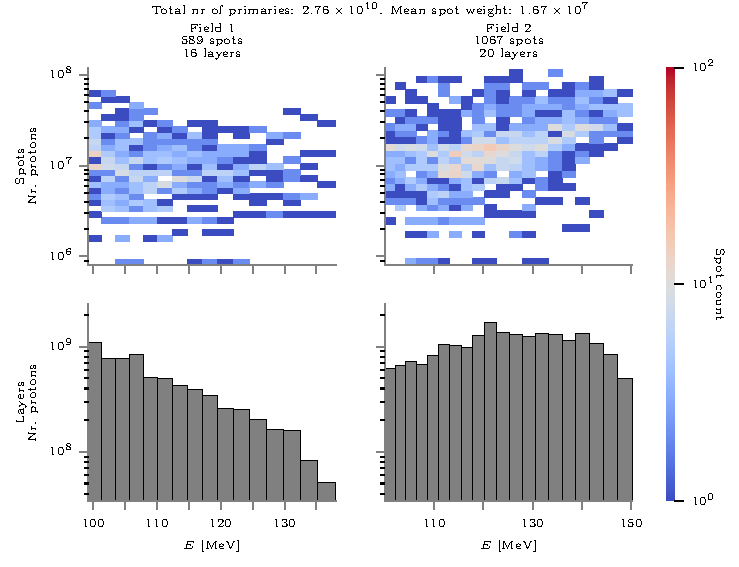
\includegraphics[width=0.9\linewidth]{plannonorm-plot}
  \caption{Structure of the 2-field treatment plan used in this study. The tumor was located in the head-and-neck region, wrapped about the trachea. In the plan shown here the first field is clearly shifted towards lower energies: this field was added to prevent field 2 from overdosing some AORs (most notably spine and optical nerves).}
  \label{fig:our-plan}
\end{figure}

\begin{figure}[htp]
  \centering
  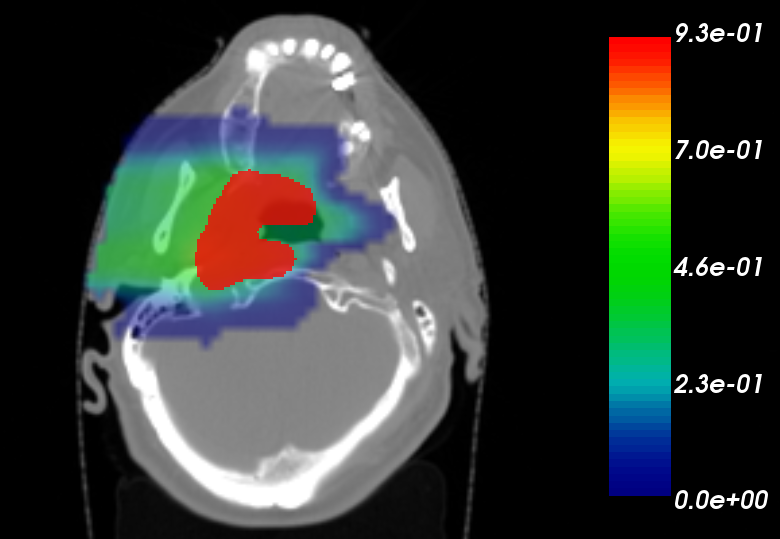
\includegraphics[width=0.5\linewidth]{ourpatient}
  \caption{A slice of the CT used in this study is shown with the dose due to field 2 of our plan overlaid, with in red the PTV structure.}
  \label{fig:our-patient}
\end{figure}

\subsection{Data selection and analysis}

\subsubsection{Fall-off position estimation procedure}\label{sec:fopproc}

Publications sometimes mix up range estimation and FOP estimation. The first requires more than the estimate of where the primary particle stops: the primary point of entry into the patient (a "fall-in" position or FIP) must also be measured, as was mentioned in \cite{Pinto2014a} as the entrance position. Of course, range estimation requires that both positions are within the field of view (FoV) of the detector, which not every proposed PG camera is capable of. The KES camera has a more limited FoV, which is why we chose to only estimate the fall-off. Note that the FIP may be estimated by other means: the optical patient positioning systems present in most clinics could be used to get the FIP, although they do not provide a direct measurement. The range estimate could be more interesting than FOP from a clinical perspective. Consider the simple case where a patient was set up a centimeter further along the beam-line: the fall-off will have shifted, but the range remains unaltered. In the case studied in here, a large part of the patient's morphological change was weight loss in the subcutaneous layer. This implies a shift of the whole ion path, but not necessarily a change in range.

\begin{figure}[htp]
  \captionsetup[subfigure]{labelformat=empty}
  \centering
  \subfloat[]{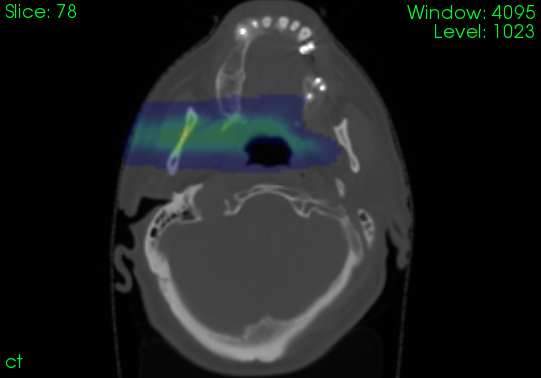
\includegraphics[width=.45\textwidth]{outpatient-pgemis-distisodepth}}\quad\quad\quad
  \subfloat[]{\includegraphics[width=.45\textwidth]{camelback}}
  \caption{Left: CT with the PG production image of the most distal iso-depth layer of the second field of our TP in fig.~\ref{fig:our-plan}. Right: the PG production profile (along the beam) of the same layer. A ragged plateau region due to inhomogeneities is sometimes called the camelback.}
  \label{fig:camelback}
\end{figure}

The guiding design principle behind collimated PG cameras is then range or FOP estimation: a 1D PG production profile is obtained, from which the FOP is extracted. Multiple approaches to extracting a FOP from the line profile have been proposed \citep{Smeets2012,Gueth2013,Roellinghoff2014a,Janssen2014,Sterpin2015}. In figure~\ref{fig:camelback} the peaks in the profile due to inhomogeneity are seen. Such a ragged plateau region is sometimes called camelback. %The concept of a single range, or FOP, per spot does not hold up in laterally inhomogeneous targets. 
No conventional fit procedure accounts for such situations. In preparatory work, we investigated a number of the proposed procedures, and all required significant tweaks to be able to deal with our data. In addition, insofar the methods had free parameters, we established significant sensitivity to such parameters on the final FOP estimates. In summary, the FOP estimate depends greatly on the procedure, the robustness relies on having yields uncommon on the spot-level in clinical TPs, and also on an absence of unavoidable inhomogeneities.

We will therefore not focus on the fitting procedure, but employ a simple method that visually works on most data we have. Our procedure is as follows:

\begin{enumerate}[noitemsep]
\item The measured PG profile is smoothed and interpolated with a smoothing spline function:

\begin{equation}
\sum_{i=1}^n (Y_i - \hat f(x_i))^2 + \lambda \int_{x_1}^{x_n} \hat f''(x)^2 \,dx
\end{equation}

where $Y_i$ is the measured PG profile and $x_i$ the associated x-coordinates, $\hat f(x_i)$ the estimate smoothed spline function and $\lambda$ a smoothing parameter that determines the penalty for deviating from measurement in exchange for smoothness (second order derivatives are close to zero on smooth functions). $\lambda = 0$ produces a perfect spline fit to the data, while $\lambda \gg 1$ produces a horizontal line. We found that $\lambda = 2$ struck the right balance between overfitting to noise and removing too many features, which tends to happen for low statistic measurements.
\item The obtained function is plotted for 1024 $x_j$. Any $f(x_j) < 0$ are set to $0$. 
\item The global maximum is found.
\item The baseline is set equal to the lowest 25\% of bins.
\item From the distal end backwards, the first maximum is taken as the distal most peak position, if it is above the threshold of 30\% of the difference between baseline and global maximum. If no such point is found, the global maximum is taken as the distal most maximum.
\item The fall-off amplitude (FOA) is set to the difference between the distal maximum and baseline: $FOA = max-baseline$. The FOP is obtained by traversing the smoothed profile from the distal end towards the peak until $y_j > \frac{1}{2}FOA$.
\end{enumerate}

The results of this procedure are illustrated in figure~\ref{fig:our-fit}. Every PG profile was estimated 50 times, and so we obtained 50 estimates for the FOP. We assume that the FOPs follow a Gaussian distribution, so the mean of the 50 realizations gives us the best FOP estimate and the sigma gives the precision of the ability to estimate the best FOP. Comparing the 50 FOP estimates obtained from the CT with the 50 estimates obtained from the RPCT simulations, gives 2500 possible shift estimates. Again, the distribution of shifts should be centered at the true shift, while the sigma tells us how likely it is that this true shift is detected under the current conditions.

\begin{figure}[htp]
  \centering
  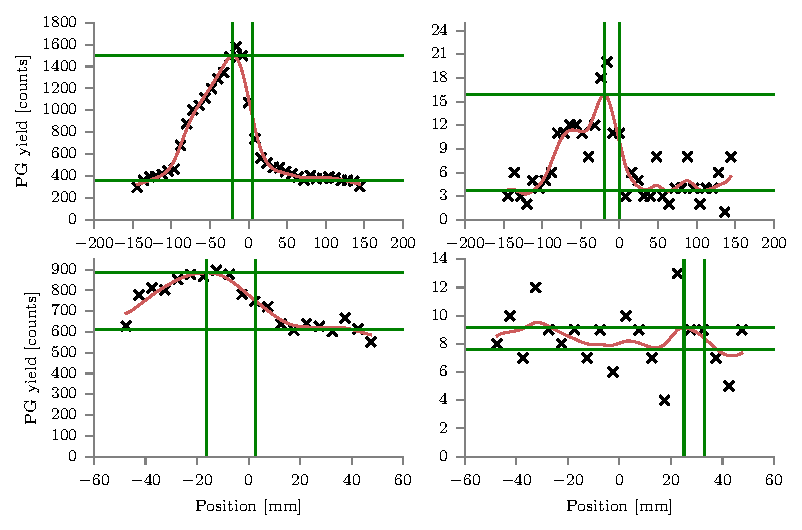
\includegraphics[width=0.99\linewidth]{fopproc}
  \caption{The top row demonstrates the fall-off determination procedure on the multi-parallel camera data; on the bottom row on knife-edge slit camera data. The left column is produced with a PG signal due to $10^9$ primaries, while the right column was produced with $10^7$ primary protons. In black crosses the measured PG counts are plotted. The smoothed data is shown in red. The green horizontal lines are drawn at the obtained distal maxima and baselines, while the vertical green lines shown the position of the distal maximum and the position of the fall-off. For the bottom-right plot, a history is visible where the procedure fails: the background induces an erroneous peak detection.}
  \label{fig:our-fit}
\end{figure}

\subsubsection{Spot selection}

\begin{figure}[htp]
  \captionsetup[subfigure]{labelformat=empty}
  \centering
  \subfloat[]{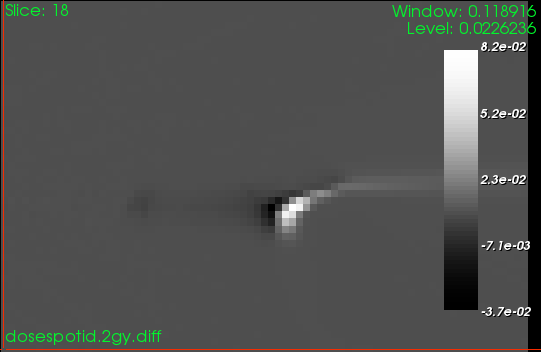
\includegraphics[width=.35\textwidth]{no-single-range-spot60-scale}}\quad\quad\quad
  \subfloat[]{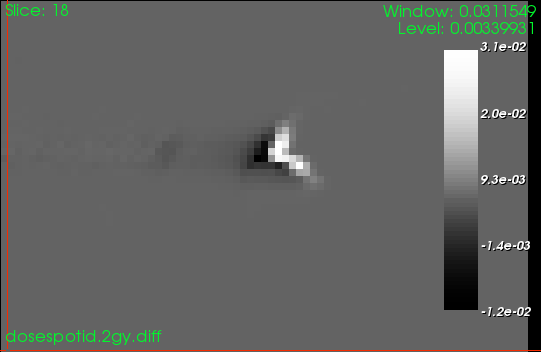
\includegraphics[width=.35\textwidth]{no-single-range-spot361-scale}}
  \caption{Axial slices of dose difference images for spots 60 and 361 demonstrate the effect of patient inhomogeneity on the range. The color scale was set to make the under- and overshoot regions clearly visible. We used a threshold to select "single range" FOPs by requiring that 20\% of FOA and 80\% of FOA are spaced out no more than 8 mm of 50\% FOA. The proton beam is entering from the left.}
  \label{fig:no-single-range}
\end{figure}

To understand the feasibility of spot FOP verification in clinical setting, it must be established how the quality of the shift estimate depends on the number of primaries per spot. We used two things in this search: the FOP estimation procedure detailed in the previous section, \emph{executed on the dose image}, and a quality-of-fit estimation. The quality of fit estimation consists of testing if the FOPs at 50\% is within a certain distance dx of the FOP evaluated at 20\% of FOA and 80\% of FOA. dx was set to 8 mm. An observation is that about 10\% of spots do not pass the uniform FOP criterion: figure~\ref{fig:no-single-range} shows two examples of the more typical case where inhomogeneities show their impact. For the spot-grouping procedure, 123 out of 1067 spots not meeting this criterion were discarded.

\begin{figure}[htp]
  \captionsetup[subfigure]{labelformat=empty}
  \centering
  \subfloat[Axial slice of the absolute dose difference for spot 61 of our TP, color scale chosen for best visibility. A relatively uniform forward shift may be observed.]{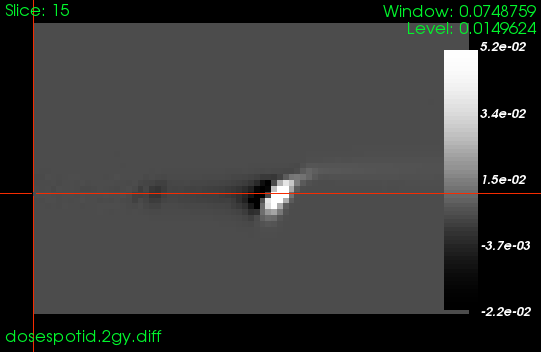
\includegraphics[width=.35\textwidth]{no-single-range-spot61-scale}}\quad\quad\quad
  \subfloat[Dose difference profile at the central line (shown in red on the left) of spot 61.]{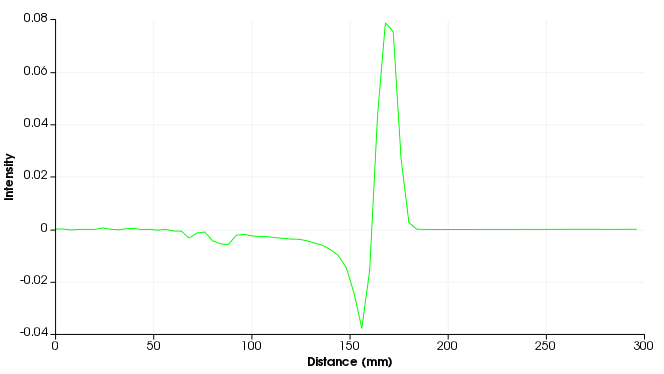
\includegraphics[width=.35\textwidth]{spot61-profile}}
  \caption{On the left the dose difference between CT and RPCT as seen from the top generated by irradiating spot 61. On the right the line profile corresponding to the red line (left).}
  \label{fig:spot61}
\end{figure}

We ended up choosing three spots (table~\ref{table:spotselec}). Spot 61, with a large shift of over a centimeter is shown in figure~\ref{fig:spot61}. Slightly visible on the right is a whiff of overshoot: the beam partially exits the patient causing the distal elevation seen in figure~\ref{fig:the-spots}. An expected shift of over a centimeter should be reliably detectable for any PG camera. Spots 29 and 40 are more challenging; with expected shifts between 2 and 4 mm they represent a minimum shift that we hope PG cameras can detect.

\begin{figure}[htp]
  \centering
  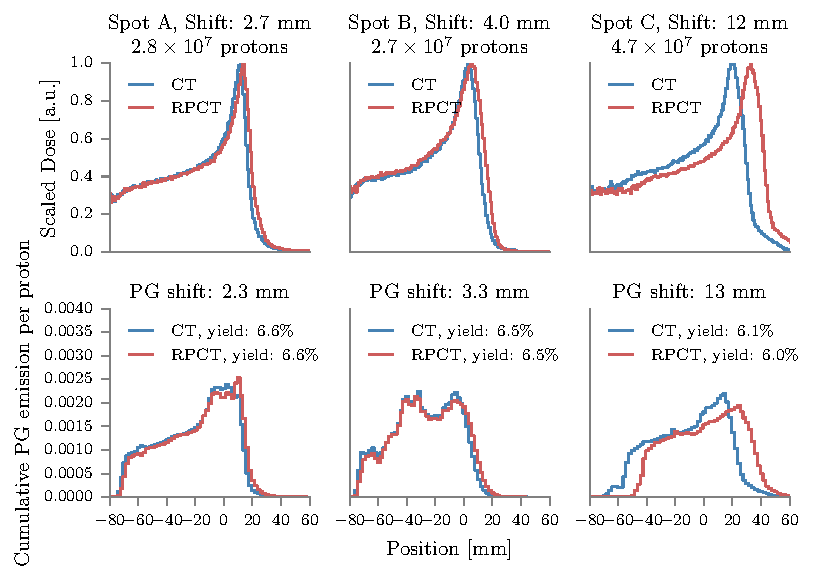
\includegraphics[width=0.99\linewidth]{spotprofiles}
  \caption{The three chosen spots, based on their shifts and quality of shift. Dose is normalized by mass, which explains the lack of structure. Top row: dose profiles, bottom row: PG profiles as used in the simulation. The yield is the integral yield of the whole image, so 6\% means 6 out of 100 protons would generate a PG.}
  \label{fig:the-spots}
\end{figure}

\begin{table}
\centering
\begin{tabular}{llll}
	 & Spot 29 & Spot 40 & Spot 61\\
	\midrule
	Dose shift [mm] & 2.77 & 4.08 & 12.4\\
	PG emission shift [mm] & 2.32 & 3.34 & 13.9\\
	PG + PSF shift [mm] & 2.61 & 2.91 & 11.9\\
	\midrule
	Iso-energy layer [MeV] & 145.86 & 143.02 & 143.02 \\
	x-pos [mm] & -24.0 &  -24.0 &  -24.0 \\
	y-pos [mm] & 16.0 & 40.0 & -40.0 \\
	Nr. protons & $2.75\cdot10^7$ & $2.72\cdot10^7$ & $4.73\cdot10^7$ \\
\end{tabular}
\caption{Summary of the properties of the selected spots.}
\label{table:spotselec}
\end{table}

%we dont do this.
%\subsubsection{Deformation Tool}
%
%Build a CLITK tool that takes an image as input, a location, size and standard deviation for the deformation. Output an image with a spherical deformation around that point with that size, and vary with the given randomness. I have a basic idea of how to start.

\subsubsection{Spot grouping}

As established in section~\ref{sec:tpanalysis}, we expect a difference between the number of protons per spot as planned and sufficient for reconstruction. Depending on the beam line, the minimum unit of PG detection may be a spot (beam scanning) or an iso-energy layer (passive scattering). Since most new centers are of the beam scanning type, we propose an alternative spot grouping method. Our assumption is that due to inhomogeneities, protons within an iso-energy layer may have very different FOPs in the patient. We will compare grouping by iso-energy layer to grouping based on expected spot FOP. On the planning CT the 3D dose distribution is computed per spot, and then a dose FOP is determined with the same algorithm as for PG FOP, see section~\ref{sec:fopproc}. We made the choice to use the dose FOP and not PG FOP because that is what is available as an output in TPS: dosemaps. In future TPSes, it may be imagined the (per spot) FOP could be output directly for applications such as PG monitoring.

The FOPs for each spot are binned along the beam line, and these bins we call iso-depth layers (red line in fig.~\ref{fig:geolayers}). In terms of proton numbers (green line), this yields similar impressions as the layer views in figure \ref{fig:planning}: the distal layer(s) have higher spot statistics but lower cumulative (layer) statistics.

\begin{figure}[htp]
  \centering
  \includegraphics[width=0.7\linewidth]{{{rtplan.geolayers}}}
  \caption{For the main field in the TP, per spot, a FOP is computed and binned (red, left y-axis). The depth dose distribution is overlaid in blue in linear arbitrary scale, as a reference for the shape. In green each spot is weighted with its number of protons (right y-axis) and then summed. With respect to the red line, the green line flattens out the top in the forward direction, supporting the thesis that in the geometric domain as well as the energy domain, the distal spots are individually weightier. However the cumulation of all spots leads to a larger dose in the medial layers of the target volume.}% but cumulatively less than medial bins or layers.}
  \label{fig:geolayers}
\end{figure}

\subsubsection{Figures of Merit}\label{figmerit}

When evaluating the detector, principally we care about accuracy and precision: does the PG camera estimate the FOP consistently correct and does it so reliably over the course of a number of experiments? A more clinical point of view could be: does the detector correctly signal significant changes? A precise FOP estimate or FOP shift estimate is perhaps not required, but a correct indication of significant change \emph{is}.

Employing the batch method we realize between 20 and 50 simulations for each experiment, each resulting in a FOP estimate, giving us a mean $\upmu_\textrm{FOP}$ and a standard deviation $\upsigma_\textrm{FOP}$ for a certain experiment. Since we are studying the effect of replacing the CT with a RPCT to simulate patient change, we run each experiment with both CT and RPCT. Each FOP estimate of the N CT realizations is compared to each FOP estimate of the N RPCT realizations, resulting in N$\times$N possible \emph{FOP shift} measurements. These distributions have a $\upmu_\Delta$ and a $\upsigma_\Delta$. The shift initially obtained with the dose is denoted $\Delta_\textrm{dose}$

%These will be compared to the $FOP_{em}$: the FOP shift obtained from the PG emission profiles, which are prepared for each spot.

Grading the performance of the detectors will be done according to a few figures of merit: 

\begin{itemize}[noitemsep]
\item Accuracy: $| \upmu_{\Delta} - \Delta_\textrm{dose}|$.
\item Precision: $\upsigma_\Delta$. For this estimate of the standard deviation of the Gaussian distribution a standard deviation can be computed once again based on the number of realization $n$ used to obtain it: $\upsigma(\upsigma_\Delta)=\frac{\upsigma_\Delta}{\sqrt{2\times(n-1)}}$, as per \citet[formula 4.54]{Leo1994}.
\item Confidence: the percentage of RPCT FOP realizations that fall outside $\upmu_\textrm{FOP,CT}\pm2\upsigma_\textrm{FOP,CT}$ indicates the likelihood any difference from the expected FOP is measured. In other words, given that in this analysis we know that a shift should be detected, what is the probability we will? It will be denoted as P$_\Delta$.

%\item Accuracy: is $| \mu_{\Delta} - \Delta_{em}|$ < 2mm?
%\item Shift measurement reliability $c_v$
%\item[] This may be quantified by the \emph{coefficient of variation} $c_v = \frac{\sigma}{\mu}$: the ratio of the standard deviation over the mean is a measure for the repeatability of an experiment. If more than one, the signal is lower than the noise and consistent results cannot be expected. Obviously, this quantity ceases to be meaningful close to zero, but both in this setup and our clinical case, we think that we are far enough from a near-zero shift that the use of $c_v$ is acceptable.
%\item Shift precision p$_\textrm{shift}$
%\item[] p$_\textrm{{shift}} = \upsigma$. It tells us if there is a 68\% chance or better to get a measurements with sub-millimeter precision.
%\item Probability of clinical relevance P$_{\textrm{cr}}$
%\item[] Apart from an accurate or precise FOP or FOP shift estimate, simply finding \emph{a} shift when there is one could be informative in itself. At the root of this indicator lies the idea that overestimating the FOP shift is less of a problem than underestimating it, if all we are interested in is having a signal that something is changed. By integrating the FOP shift distribution from a threshold value and upwards, we obtain $_{\textrm{cr}}$. As a threshold, we choose $\upmu - 1$mm, which means any shift over $\upmu - 1$mm an is acceptable indicator that \emph{a} change was present. For sharp distributions, P$_{\textrm{cr}} = 1$; for broad distributions P$_{\textrm{cr}}$ converges to $\frac{1}{2}$.

%The cumulative distribution function for a normal distribution with mean $\mu$ and standard deviation $\sigma$ on interval $[-\infty,x]$ is:

%\begin{equation}
%\textrm{CDF(x)} = \frac{1}{2} \bigg[ 1 + \textrm{erf} \bigg( \frac{x-\mu}{\sigma\sqrt{2}} \bigg) \bigg]
%\end{equation}

%where erf is the error function. Thus, by setting $x=\mu - \sigma$ and computing 1-CDF(x) we can compute $P_{cr}$ as:

%\begin{equation}
%\textrm{P}_{\textrm{cr}} = \textrm{CDF}(\upmu - 1\textrm{mm})
%\end{equation}

%http://mathworld.wolfram.com/NormalDistribution.html
%\item Clinical shift indicator $CSI$
%\item[] For a clinical application retrieving correct FOP shifts may be less important than establishing significant difference. Therefore, an overestimated FOP shift distribution is beneficial: we are very likely to get an indicator of change for a single realisation. $CSI = \sigma < 2mm$
\end{itemize}

\subsection{Verification of Knife-Edge results}

\begin{figure}[htp]
  \captionsetup[subfigure]{labelformat=empty}
  \centering
  \includegraphics[width=.8\textwidth]{{{waterbox-iba-auger-notof-3.root-FOP}}} %double escape dot in filename
  \caption{Knife edge FOP estimates for a simple simulation of a beam in a waterbox. In red, the beam was set at 139 MeV and 144 MeV is shown in blue. 50 realizations for each setting are overlaid, with their FOP plotted as a vertical line.}
  \label{fig:waterbox-fops}
\end{figure}

In \cite{Priegnitz2015} PG shifts due to beam energy shifts are studied. They include a study in the \emph{detectability} of the fall-off as function of the number of primaries. To test our implementation of the knife-edge camera, we recreated the simulation: we shoot a mono-energetic beam into a waterbox at two energies with a 5 MeV shift. We created 50 realizations with a 139 MeV beam energy, and 50 realizations with 144 MeV. In figure~\ref{fig:waterbox-fops} the profiles are plotted.

The results in figure~\ref{fig:waterbox} are very similar to those in \citet[figure 9]{Priegnitz2015}: at $10^9$ primaries, the distributions are well separated with a shift of 8.3 mm (different from \cite{Priegnitz2015} because of the different material). In figure 13 in \cite{Perali2014} with $10^9$ primaries a standard deviation of 1.5 mm is obtained, while we have 1.21 and 1.14 mm. We consider this sufficient agreement to be confident of our setup and further results. \cite{Roellinghoff2014a} recalls that $\upsigma_\textrm{FOP}$ is proportional to the contrast-to-noise ratio (CNR) $\frac{\sqrt{\textrm{background}}}{\textrm{signal}}$, which is proportional to $\frac{1}{\sqrt{N_\textrm{prim}}}$. That means the increase in $\upsigma$ in figure~\ref{fig:waterbox} should be roughly a factor 3 as the order of magnitude in number of primaries decreases. Between $10^8$ and $10^9$ this holds, but between $10^7$ and $10^8$ it does not, likely because of the noisiness of the profiles generated with $10^7$ primaries, on which the FOP estimation procedure is prone to misidentify the peak position.

\begin{figure}[htp]
  \captionsetup[subfigure]{labelformat=empty}
  \centering
  \includegraphics[width=.8\textwidth]{{{waterbox-iba-auger-notof-3.root-FOP-dist}}} %double escape dot in filename
  \caption{Knife edge FOP estimates for a simple simulation of a beam in a waterbox. In blue, the beam was set at 139 MeV and 144 MeV is shown in red. The CNR test holds between $10^8$ and $10^9$ holds, but between $10^7$ and $10^8$ it does not.}
  \label{fig:waterbox}
\end{figure}

%\subsubsection{Camera alignment}

Note that the Knife-Edge prototype is very sensitive to accurate positioning with respect to the expected FOP. This was elaborated upon in \citet[Section IV.A.3]{Sterpin2015}: the detector response is, due to the KES collimator, not linear as with a parallel slit collimator. The response further away from the position directly in front of the KES slit is slightly lower due to the increased photon path length through the patient and the attenuation incurred by that longer path. Additionally, the solid angle per detector pixel depends on the position with respect to the KES slit. Initially we aligned the camera at the isocenter, which may be tens of centimeters away from the KES slit. We confirm the observation that this results in incorrect FOP estimates, for our spot 61 of up to half a centimeter. For clinical cases, alignment with the FOP from the TPS dose profile may be a workable alternative. In this study, to make the comparison as fair as possible and avoid any bias, alignment on the FOP specific for each spot was done as follows: the intermediate PG source image of vpgTLE (equivalent to the PG emission) was projected on the beam axis, and then convolved with a Gaussian of $\upsigma = 8.5$ mm, which corresponds to the point spread function (PSF) with a FWHM of 20 mm used in \cite{Priegnitz2015} to approximate the detected profiles from the emitted profile. %For Gaussians the FWHM is related to the $\upsigma$ as follows: $\mathrm{FWHM} = 2\sqrt{2 \ln 2 } \; \upsigma \approx 2.355 \; \upsigma \leadsto \upsigma \approx \frac{20}{2.355} \approx 8.5$.

%\cite{Richter2016} mentions that the range of the field (dose we presume) is the leading 

\subsection{Verification of Multi-Parallel Slit results}

\begin{figure}[htp]
  \captionsetup[subfigure]{labelformat=empty}
  \centering
  \includegraphics[width=.8\textwidth]{{{waterbox-ipnl-auger-tof-1.root-FOP}}} %double escape dot in filename
  \caption{Multi parallel slit FOP estimates for a simple simulation of a beam in a waterbox. In red, the beam was set at 139 MeV and 144 MeV is shown in blue. 50 realizations for each setting are overlaid, with their FOP plotted as vertical lines.}
  \label{fig:waterboxipnl-fops}
\end{figure}

\begin{figure}[htp]
  \captionsetup[subfigure]{labelformat=empty}
  \centering
  \includegraphics[width=.8\textwidth]{{{waterbox-ipnl-auger-tof-1.root-FOP-dist}}} %double escape dot in filename
  \caption{Multi parallel slit FOP estimates for the same setup used to verify the Knife Edge results: a beam in a waterbox. In blue, the beam was set at 139 MeV and 144 MeV is shown in red. The CNR test holds when comparing $\upsigma$s for $10^8$ and $10^9$ primaries, but again the profiles for $10^7$ were too noisy to produce reliable FOP estimates.}
  \label{fig:waterboxipnl}
\end{figure}

As a verification our implementation of the MPS camera, we checked that we obtain a similar precision on the FOP by repeating the procedure performed for the KES (fig.~\ref{fig:waterboxipnl-fops}). In the caption of figure 9 in \cite{Pinto2014a} we read that with $10^8$ primaries a standard deviation of 1.3 mm for the detector design used here is obtained, which is about 20\% different from our 1.63 and 1.54 mm in figure~\ref{fig:waterboxipnl}.

%As a verification our implementation of the MPS camera, we checked that we obtain a similar precision on the FOP. Table 6 in \cite{Pinto2014a} shows this to be 0.59(0.06) for $5\cdot10^8$ primaries, while we obtain sigmas of 0.46-0.81 using $10^9$ primaries (spot 29 RPCT and spot 61 RPCT respectively). The obvious difference is the inhomogeneity of the target, which was assumed to have no effect towards the FOP [TODO: CITATION NEEDED].

%FOP precision: \cite{Pinto2014a} Table 6 case 1: $0.59mm$ at $10^9$ prims, homogeneous phantom. We seem to have about $0.7mm$, for different spots, so a confirmation of the result and of the thesis that inhomoheneities don't affect the PG camera performance. %no need for fading in ct study
A last number perhaps of interest is the detection yield: we saw an average of $2.5\cdot10^{-5}$ detections per emitted PG for the MPS camera, and around $1.5\cdot10^{-5}$ for the KES. In combination with the number of detector bins (MPS: 37, KES: 20), these numbers help understand why $10^6$ primaries can be dismissed right off the bat: a reasonable profile can never be estimated with a handful of counts. Therefore we omitted the $10^6$ data from the analysis. The CNR test holds when comparing $\upsigma$s for $10^8$ and $10^9$ primaries, but again the profiles for $10^7$ were too noisy to produce reliable FOP estimates.


%%%%%%%%%%%%%%%%%%%%%%%%%%%%%%%%%%%%%%%%%%%%%%%%%%%%%%%%%%%%%%%%%%%%%%%%%%%%%%%%%%%%%%%%%%%%%%%%%%%%%%%%%%%%%%%%%%%%%%%%%%%%%%%%%%%%%%%%%%%%%%%%%%%%%%%%%%%%%%%%%%%%%%%%%%%%%%%%%%%%%%%%%%%%%%%%%%%%%%%%%%%%%%%%%%%%%%%%%%%%%%%%%%%%%%%%%%%%%%%%%%%%%%%%%%%%%%%%%%%%%%%%%%%%%%%%%%%%%%%%%%%%%%%%%%%%%%%%%%%%%%%%%%%%%%%%%%%%%%%%%%%%%%%%%%%%%%%%%%%%%%%%%%%%%%%%%%%%%%%%%%%%%%%%%%%%%%%%%%%%%%%%%%%%%%%%%%%%%%%%%%%%%%%%%%%%%%%%%%%%%%%%%%%%%%%%%%%%%%%%%%%%%%%%%%%%%%%%%%%%%%%%%%%%%%%%%%%%%%%%%%%%%%%%%%%%%%%%%%%%%%%%%%%%%%%%%%%%%%%%%%%%%%%%%%%%%%%%%%%%%%%%%%%%%%%%%%%%%%%%%%%%%%%%%%%%%%%%%%%%%%%%%%%%%%%%%%%%%%%%%%%%%%%%%%%%%%%%%%%%%%%%%%%%%%%%%%%%%%%%%%%%%%%%%%%%%%%%%%%%%%%%%%%%%%%%%%%%%%%%%%%%%%%%%%%%%%%%%%%%%%%%%%%%%%%%%%%%%%%%%%%%%%%%%%%%%%%%%%%%%%%%%%%%%%%%%%%%%%%%%%%%%%%%%%%%%%%%%%%%%%%%%%%%%%%%%%%%%%%%%%%%%%%%%%%%%%%%%%%%%%%%%%%%%%%%%%%%%%%%%%%%%%%%%%%%%%%%%%%%%%%%%%%%%%%%%%%%%%%%%%%%%%%%%%%%%%%%%%%%%%%%%%%%%%%%%%%%%%%%%%%%%%%%%%%%%%%%%%%%%%%%%%%%%%%%%%%%%%%%%%%%%%%%%%%%%%%%%%%%%%%%%%%%%%%%%%%%%%%%%%%%%%%%%%%%%%%%%%%%%%%%%%%%%%%%%%%%%%%%%%%%%%%%%%%%%%%%%%%%%%%%%%%%%%%%%%%%%%%%%%%%%%%%%%%%%%%%%%%%%%%%%%%%%%%%%%%%%%%%%%%%%%%%%%%%%%%%


\section{Results}

The first study is on the performance of the two collimated PG camera designs on a patient case with a CT and follow-up CT. Secondly, we investigate how two PG cameras perform as function of the number of primaries for a given spot. To conclude, we propose a new spot-summing method, we discuss why it's an improvement over iso-energy layer summing, and demonstrate its effect.

%inspiration: \cite{Schmid2015} ?

% - important to show dose differences, DVH, gamma index, dosemap (select slice with VV?)
% 	- take diff of dose, overlay on CT with proper scale.
% 	- DVH tool: ask Thomas
% 	- gamma index, consider >90% max dose, count percentage pixel gammaindex >1, <1

\subsection{Weight-modulated single spot}

%PG FOPS
%pg29 13.7694140625 , w/psf: 19.44421875
%rppg29 16.0975390625 , w/psf: 22.063359375
%pg40 4.8934375 , w/psf: 8.5311328125
%rppg40 8.2401171875 , w/psf: 11.4412890625
%pg61 22.2088671875 , w/psf: 29.047734375
%rppg61 36.1776171875 , w/psf: 40.979375
%FOP shifts
%29, ct: 2.77 , pg 2.32 , pg+psf 2.61
%40, ct: 4.08 , pg 3.34 , pg+psf 2.91
%61, ct: 12.4 , pg 13.9 , pg+psf 11.9


%ideas for figures of merit:
%\begin{itemize}[noitemsep]
%\item plot dose diffs: beam eye view (BEV, along beam) 2D plot with in color the range shifts. Fig 4, Hudobivnik et al.
%\item gamma map slice + histogram, 2\%/2mm, not 3/3.
%\item dose diff slice + histogram (Joris)
%\end{itemize}
%plot dose diffs: beam eye view (BEV, along beam) 2D plot with in color the range shifts. Fig 4, Hudobivnik et al.

\begin{figure}[htp]
  \captionsetup[subfigure]{labelformat=empty}
  \centering
  \subfloat[MPS, spot 29]{\includegraphics[width=.49\textwidth]{{{spot29-ipnl-auger-tof-1.root-FOP-shift}}}}\quad
  \subfloat[KES, spot 29]{\includegraphics[width=.49\textwidth]{{{spot29-iba-auger-notof-3.root-FOP-shift}}}}\quad
  \subfloat[MPS, spot 40]{\includegraphics[width=.49\textwidth]{{{spot40-ipnl-auger-tof-1.root-FOP-shift}}}}\quad
  \subfloat[KES, spot 40]{\includegraphics[width=.49\textwidth]{{{spot40-iba-auger-notof-3.root-FOP-shift}}}}\quad
  \subfloat[MPS, spot 61]{\includegraphics[width=.49\textwidth]{{{spot61-ipnl-auger-tof-1.root-FOP-shift}}}}\quad
  \subfloat[KES, spot 61]{\includegraphics[width=.49\textwidth]{{{spot61-iba-auger-notof-3.root-FOP-shift}}}}
  \caption{The FOP difference distributions are plotted for the spots (row-wise) and for the MPS and KES cameras (column-wise). Per subplot, four times two FOP distributions are shown. In front the FOP shifts based on $10^9$, $10^8$, the original spot weight, and $10^7$ as we go towards to back of the 3D plot.}
  \label{fig:spotshifts}
\end{figure}

The procedure outlined in section~\ref{figmerit} and demonstrated in the validation stage, is performed for all number of primaries, for both cameras, for spots 29, 40 and 61. Because of the extent of the results, the intermediate steps arae presented in appendix~\ref{appspot}. The plots of the final results, the FOP shift distributions and their $\upmu_\Delta$, $\upsigma_\Delta$ and P$_\Delta$ are shown in figure \ref{fig:spotshifts}

\begin{table}
\centering
\begin{tabular}{llll}
	 & Spot 29 shift [mm] & Spot 40 shift [mm] & Spot 61 shift [mm]\\
	\midrule
	Dose & 2.77 & 4.08 & 12.4\\
	PG emission & 2.32 & 3.34 & 13.9\\
	PG + PSF & 2.61 & 2.91 & 11.9\\
	$\upmu_\Delta$ MPS @ $10^9$      & 2.68$\pm$0.77 & 3.23$\pm$0.77 & 12.6$\pm$1.15 \\
	$\upmu_\Delta$ KES @ $10^9$      & 2.56$\pm$1.93 & 3.27$\pm$2.24 & 9.79$\pm$2.25 \\
	%$\upmu_\Delta$ MPS @ $10^8$      & & & 11.6$\pm$3.25 \\
	%$\upmu_\Delta$ KES @ $10^8$      & & & 7.01$\pm$16.2 \\
	$\upmu_\Delta$ MPS @ spot weight & 2.51$\pm$4.05 & 3.76$\pm$4.36 & 12.5$\pm$4.73 \\
	$\upmu_\Delta$ KES @ spot weight & -1.2$\pm$28.9 & -0.2$\pm$28.9 & 4.30$\pm$26.2 \\
	\midrule
	 & Spot 29 P$_\Delta$ & Spot 40 P$_\Delta$ & Spot 61 P$_\Delta$\\
	\midrule
	P$_\Delta$ MPS @ $10^9$      & 99\%  & 99\% & 100\% \\
	P$_\Delta$ KES @ $10^9$      & 43\%  & 59\% & 99\% \\
	P$_\Delta$ MPS @ spot weight & 20\%  & 24\% & 96\% \\
	P$_\Delta$ KES @ spot weight & 1.9\% & 1.6\% & 1.4\% \\
	\midrule
	 & Spot 29 spot weight & Spot 40 spot weight & Spot 61 spot weight\\
	\midrule
	Nr. protons & $2.75\cdot10^7$ & $2.72\cdot10^7$ & $4.73\cdot10^7$ \\
\end{tabular}
\caption{Results from figure~\ref{fig:spotshifts} summarized and compared to the ground truths from figure~\ref{fig:the-spots}: the accuracy can be gleaned by comparing the shifts, the probability of measuring the change is estimated with P$_\Delta$. With "PG + PSF" the FOP on the PG emission profile convolved with a Gaussian with a 20 mm FWHM is indicated. The geometric effect of the detector not measuring the PGs at emissions but at detection, approximated by the convolution, leads to up or downstream shifted FOPs.}
\label{table:spots}
\end{table}

Table~\ref{table:spots} summarizes the results relevant to the ultimate estimated shifts. With $10^9$ primaries, both cameras are within 2 mm of the "PG + PSF" emission shift, except the KES camera in spot 61. Here, when its $\upsigma_\Delta$ is considered, it is within one $\upsigma$ of the expected value. At the prescribed spot weights, the MPS still converges on the correct $\upmu_\Delta$, but the KES no longer. Considering that the $\upsigma_\Delta$ for the KES is on the order of half the field of view of the camera, it seems fair to draw the conclusion no correct FOPs are estimated at these spot weights.

Turning to P$_\Delta$ at $10^9$ primaries, we observe that the MPS performs very well: for any spot the probability that a single RPCT realization indicates a change from the CT is at least 99\%. The KES reaches the same probability only for the large shift of spot 61. At their planned spot weights, neither camera provides great results except for the MPS for spot 61: even though the precision is 4.73 mm, the size of the true shift is enough to keep the CT and RPCT FOP distributions separated enough to be 96\% certain a single measurement would have provided a clue that there was a significant shift. 

%TODO: reinstate det comp?

%\subsection{Detector comparison}

%\begin{figure}[htp]
%  \captionsetup[subfigure]{labelformat=empty}
%  \centering
%  \subfloat[]{\includegraphics[width=.47\textwidth]{{{spot61-ipnl-auger-tof-1.root-FOP}}}}\quad\quad\quad
%  \subfloat[]{\includegraphics[width=.47\textwidth]{{{spot61-iba-auger-notof-3.root-FOP}}}}
%  \caption{PG yields as function of the number of primary particles in the spot. The MPS camera is the detector device on the left 4 plots, the KES camera is on the right 4 plots. Blue is the result of the CT image, red the RPCT image. For each camera, the top left is a realization of $10^9$ protons, top right $10^8$, bottom left $10^7$ and bottom right $10^6$.}
%  \label{fig:pgprim}
%\end{figure}

%In figure~\ref{fig:pgprim} the PG profiles are plotted for a realization of a simulation on the PCT (blue) and RPCT (red), for the MPS camera (left), the KES camera (right) and for $10^9 - 10^6$ primaries. This is data our FOP method operates on (fig.~\ref{fig:our-fit}). The two cameras have different parameters, perhaps most obviously the FoV. As explained in section~\ref{sec:camera}, we compared the camera as specified in their respective publications.

%However, we can easily adapt ToF and energy window selections, so we will compare the $\mu$, $\sigma$ and $c_v < 1$ for each combination of ToF and energy window, for each camera and each number of primaries. We assume that ToF selection only has an effect on the background component. To remove the noise reduction for the MPS camera, we therefore increase the mean background level with $\frac{1}{0.4} = 2.5$ (where 0.4 is the ToF window with respect to the beam period ($\frac{4 ns}{10 ns}$). For the KES camera, we reduce the background with a factor 2.5 to simulated the same ToF selection window.

%\begin{tabular}{llllllllllllll}
%	&	&ToF	&	&	&	&	&	&no ToF	&	&	&	&	&\\
%	&	&1-8	&	&	&3-6	&	&	&1-8	&	&	&3-6	&	&\\
%	&	&$\mu$	&$\sigma$	&$c_v$	&$\mu$	&$\sigma$	&$c_v$	&$\mu$	&$\sigma$	&$c_v$	&$\mu$	&$\sigma$	&$c_v$\\
%MPS	&$10^9$	&4,6	&1,3	&\checkmark	&5,4	&2,4	&<1	&5	&1,4	&<1	&5,1	&2,7	&<1\\
%	&$10^8$	&3,3	&5,3	&	&5	&7,7	&	&3,8	&5,7	&	&5,7	&6,9	&\\
%	&$10^7$	&3,8	&14	&	&8,7	&76	&	&3,7	&49	&	&0,5	&81	&\\
%	&$10^6$	&4,4	&89	&	&-12	&74	&	&32	&83	&	&3,5	&81	&\\
%KES	&$10^9$	&2,3	&1,3	&<1	&2,1	&1,8	&<1	&2,5	&1,1	&<1	&1,8	&2,8	&\\
%	&$10^8$	&1,4	&3,3	&	&3,5	&5,7	&	&0,7	&4	&	&5,6	&7,4	&\\
%	&$10^7$	&3,2	&11	&	&-4	&19	&	&3,7	&15	&	&0	&20	&\\
%	&$10^6$	&6,1	&27	&	&2,4	&28	&	&4,2	&25	&	&5,8	&28	&\\
%\end{tabular}

\subsection{Spot grouping}

%PG FOPS
%pgelay_fo 15.37 , w/psf: 19.0076953125
%rppgelay_fo 22.4998828125 , w/psf: 23.9549609375
%pggeolay_fo 18.571171875 , w/psf: 23.5184375
%rppggeolay_fo 25.7010546875 , w/psf: 29.7752734375
%FOP shifts
%ELAY, ct: 6.40 , pg 7.12 , pg+psf 4.94
%GEOLAY, ct: 7.27 , pg 7.12 , pg+psf 6.25

Since spot-by-spot FOP shift measurements appear to be off the table, we can consider collecting data during the delivery of multiple spots. Based on the spot modulation analysis, the minimum proton count required should be no less than $10^9$ primaries. We take spot 61 as a start, which is conveniently part of the first iso-energy layer (counted down from highest energy) having at least $10^9$ protons. The geometric group is constructed by grouping spots with FOPs closest to spot 61's FOP until $10^9\pm5\%$ protons is reached. The final count is $1.07\cdot10^9$ and $0.98\cdot10^9$ protons in the iso-energy and iso-depth layers respectively.

%1068263318 979533764
\begin{figure}[htp]
  \captionsetup[subfigure]{labelformat=empty}
  \centering
  \subfloat[PG emission]{\includegraphics[width=.69\textwidth]{{{layprofiles}}}}\quad
  \subfloat[MPS, FOP distribution]{\includegraphics[width=.49\textwidth]{{{layer61-ipnl-auger-tof-1.root-FOP-dist}}}}\quad
  \subfloat[KES, FOP distribution]{\includegraphics[width=.49\textwidth]{{{layer61-iba-auger-notof-3.root-FOP-dist}}}}\quad
  \subfloat[MPS, FOP shift distribution]{\includegraphics[width=.49\textwidth]{{{layer61-ipnl-auger-tof-1.root-FOP-shift}}}}\quad
  \subfloat[KES, FOP shift distribution]{\includegraphics[width=.49\textwidth]{{{layer61-iba-auger-notof-3.root-FOP-shift}}}}
  \caption{On top the PG emission profile (along the beam) is shown: left the iso-energy and right the iso-depth spot groupings, again in blue the CT and red the RPCT. On the second row, we see the FOP distributions with on the left the MPS and the right the KES results. The bottom row shows the FOP shift distributions.}
  \label{fig:grouping61}
\end{figure}

Observing figure~\ref{fig:grouping61}, we see the fall off region is narrower, steeper and more regular with iso-depth grouping. Because of the sparse number of spots around spot 61, the grouped spots have dose FOPs of up to 9 mm different from spot 61. Altogether the iso-energy and iso-depth grouping share 30\% the same spots. The camelback in the iso-depth profiles may be explained by this spread in FOPs. The iso-energy RPCT shows a clear partial forward shift with a shoulder right around the middle of the fall-off, which may translate to spread in the obtained FOPs. The fall-off slopes in the iso-depth profiles are different, which is reflected in second row of the figure: a larger $\upsigma_\Delta$ for the RPCT is obtained. If we consider that spot 61 and spot 40 are both part of the energy layer, with very different FOPs, but the $\upsigma_\textrm{FOP}$ is preserved. Averaged over spots 40 and 61, CT and RPCT, $\upsigma_\textrm{FOP}$ is 0.56 and 1.58 mm for the MPS and KES respectively, while averaged over iso-depth and iso-energy grouping and CT and RPCT, $\upsigma_\textrm{FOP}$ is 0.78 and 2.4 mm resp. For the KES, $\upsigma_\textrm{FOP}$ is consistently better with iso-depth grouping however (averaged over CT and RPCT: 2.02 and 2.69 mm for iso-depth and iso-energy resp.).

\begin{figure}[htp]
  \captionsetup[subfigure]{labelformat=empty}
  \centering
  \subfloat[PG emission, spot 29]{\includegraphics[width=.49\textwidth]{{{layprofiles29}}}}\quad
  \subfloat[PG emission, spot 40]{\includegraphics[width=.49\textwidth]{{{layprofiles40}}}}\quad\quad\quad
  \subfloat[MPS, FOP shift distribution, spot 29]{\includegraphics[width=.49\textwidth]{{{layer29-ipnl-auger-tof-1.root-FOP-shift}}}}\quad
  \subfloat[KES, FOP shift distribution, spot 29]{\includegraphics[width=.49\textwidth]{{{layer29-iba-auger-notof-3.root-FOP-shift}}}}\quad\quad\quad
  \subfloat[MPS, FOP shift distribution, spot 40]{\includegraphics[width=.49\textwidth]{{{layer40-ipnl-auger-tof-1.root-FOP-shift}}}}\quad
  \subfloat[KES, FOP shift distribution, spot 40]{\includegraphics[width=.49\textwidth]{{{layer40-iba-auger-notof-3.root-FOP-shift}}}}
  \caption{In top left the PG emission profiles are plotted for groups about spot 29, with iso-energy and iso-depth groups far left and center left respectively. On the right, the same plots for the groupings about spot 40. Blue lines show the CT PG emission, red the RPCT PG emission.
  The middle row shows the FOP shift distributions for the two grouping methods for the iso-energy and iso-depth (both with $0.84\times10^9$ primaries) groups about spot 29. The bottom row shows the results for the spot grouping about spot 40, with $1.07\times10^9$ primaries for both groupings. For either row the left results were obtained with the MPS camera and those on the right with the KES camera. }
  \label{fig:groupingother}
\end{figure}

If we make the iso-depth and iso-energy groups based on spots 29 and 40, the plots in figure~\ref{fig:groupingother} are obtained. Now, the number of primaries per grouping are nearly identical between the groupings ($0.84\cdot10^9$ for the spot 20 groupings and $1.07\cdot10^9$ for the spot 40 groupings). The lower number of primaries is reflected in the $P_\Delta$ for both cameras: both are no longer at a steady 99\% as with the spot 61 groupings, but less. The small shift of spot 29 translates to small shifts in the groupings, especially the iso-depth grouping. Here, the FOP shift is well within the precision of the KES camera, and so it clearly loses its power to discriminate the CT signal for the RPCT ($P_\Delta$ = 14\%). The MPS shows, apart from the iso-energy group about spot 29, a slight improved on the $\upmu_\Delta$ when compared to the spot set to $10^9$ protons. For each camera and spot, the precision on the FOP difference ($\upmu_\Delta$) improves with iso-depth over iso-energy grouping.

\begin{table}
\centering
\begin{tabular}{lllllll}
	 & Spot 29 & & Spot 40 & & Spot 61\\
	 & iso-energy & iso-depth & iso-energy & iso-depth & iso-energy & iso-depth \\
	\midrule
	Dose & 2.47 & 1.60 & 6.40 & 4.07 & 6.40 & 6.40 \\
	PG emission & 4.94 & 2.32 & 7.12 & 3.78 & 7.12 & 7.12 \\
	PG + PSF & 3.20 & 2.18 & 4.94 & 4.51 & 4.94 & 6.25 \\
	$\upmu_\Delta$ MPS & 3.13$\pm$1.16 & 2.18$\pm$0.89 & 4.82$\pm$1.00 & 3.67$\pm$0.96 & 4.72$\pm$1.17 & 5.77$\pm$1.05  \\
	$\upmu_\Delta$ KES & 4.20$\pm$3.61 & 1.80$\pm$2.55 & 4.90$\pm$3.38 & 3.75$\pm$2.71 & 4.15$\pm$3.82 & 5.15$\pm$2.87  \\
	%\midrule
	% & iso-energy P$_\Delta$ & iso-depth P$_\Delta$ & iso-energy P$_\Delta$ & iso-depth P$_\Delta$ & iso-energy P$_\Delta$ & iso-depth P$_\Delta$ \\
	\midrule
	P$_\Delta$ MPS & 96\% & 92\%  & 99\% & 99\%  & 99\% & 99\% \\
	P$_\Delta$ KES & 34\% & 14\%  & 54\% & 57\%  & 99\% & 99\%  \\
	%\midrule
	% & Iso-energy weight & Iso-depth weight \\
	\midrule
	Nr. protons & $0.84\cdot10^9$ & $0.84\cdot10^9$ & $1.07\cdot10^9$ & $1.07\cdot10^9$ & $1.07\cdot10^9$ & $0.98\cdot10^9$ \\
\end{tabular}
\caption{Overview of the iso-energy versus iso-depth comparison: the accuracy can be gleaned by comparing the shifts, the probability of measuring the change is estimated with P$_\Delta$. All shifts are given in units of millimeters. The fact that the PG emission and dose shifts for spot 61 are exactly the same with iso-energy and iso-depth grouping is purely fortuitous.}
\label{table:layerresults}
\end{table}

%We know that the fall-off width has no effect on the precision (based on private communication with Frauke Roellinghoff), and the results summarized in table~\ref{table:layerresults} seem to confirm this: $\upsigma_\textrm{FOP}$ does not change appreciably between the two grouping methods.
Observing table~\ref{table:layerresults}, the better FOP precision of the KES for iso-depth grouping is translated to a higher probability to measure a significant change: $\upmu_\Delta$ improved from 38\% to 75\%. Looking at the groupings for spot 40, we see that the PG + PSF convolution produces a very similar FOP difference, while the FOP at PG emission and dose are quite different.

%%%%%%%%%%%%%%%%%%%%%%%%%%%%%%%%%%%%%%%%%%%%%%%%%%%%%%%%%%%%%%%%%%%%%%%
\section{Discussion}

Even though cameras with different collimators were used in this study, the goal was not to compare designs per se, but to see the differences in performance in two particular cameras both optimized for FOP precision.

\subsection{Spot 61}

The lower detection yield for spot 61 may seem puzzling at first, but may be explained with gamma attenuation in the patient. Spot 40 and 61 share a coordinate in the plane transverse to the beam, but differ because they are almost at opposite ends of the other dimension in the transverse plane, which puts spot 61 about 5 cm deeper in the patient seen from the cameras point of view. \citet[Table 3]{Lin2016} presented some results with respect to attenuation: a 10 cm increase of path lenth in a PMMA target leads to a 24\% detection yield reduction with the MPS camera of that paper, and 39\% with their KES.

\subsection{Simulation limitations}

This study was performed in silico. We used Geant4's QGSP\_BIC\_HP\_EMY physicslist to produce our results. For Geant4 is it known that currently PG production is overestimated; about 30\% according to \cite{Pinto2016}. This means that the results presented here may be better than in reality. Secondly, we have used the vpgTLE method, which only simulates PGs due to the primary protons; no background estimation is provided, which has not been subjected to calibration with empirical results in any case. The room and nozzle were not modeled. Nevertheless, background estimates were taken from the original papers, and they were both based on experimental measurement.

\subsection{Multiple fields and FOP}

Range verification is useful for under- and overshoot detection. It does not provide checks for transverse error. If there is an organ at risk (OAR) right behind the (geometrically) distal layer, FOP verification would provide valuable information. The interplay between multiple fields is difficult to disentangle, because an overshoot in one field may be compensated by an undershoot in another field, but that was considered out of scope for this publication. For single field treatment plans, or perpendicular beams where under- and overshoot or not likely to compensate, FOP verification is easily understood.

%Unlike with the spots, convoluting the PG emission profile with the Gaussian results in an appreciably different shift.
We can expect different shifts due to the profile's various shapes, changing from spot to spot, and profile differences depending on the particular grouping. %is based on various spots and range mixing causes irregularities in the profile and a wider fall-off region.
Adding the PSF blurs these features and -- apparently -- can alter the shift estimate. Range mixing is inherent to spot grouping, and therefore to altering the profile shape, so it is something to be aware of.

%\subsection{Improvements to vpgTLE}
%Use Thomas all-purpose fixed forced detection for stage 2. Then analyze where time is spent. ??

\subsection{From FOP to Range to Profile measurement}

The FOP estimation algorithm presented here was not the primary focus of the study. Possibilities for improvement are likely. As far as these authors could establish, our method was broadly similar to procedures in other publications: a maximum and a floor are extracted from the (smoothed) profile, the difference of which is the FO. Then, the FOP is set to the position where the profile crosses the half-FOA threshold. This means such procedure is sensitive to the floor and maximum estimation. With low statistics, the peak may be misidentified at a noisy bin. For the KES, incorrect alignment to the expected FOP may lead to the background falling outside of the field of view and may lead to a misidentified floor. In our plan, the width of the KES FO was about 4 cm. The angular resolution of collimated cameras implies some blurring and therefore broadening of the FO width. With a FoV of 10 cm and a possible forward shift of perhaps more than a cm (spot 61) it is not uncommon that little if any post BP floor is in the FoV. Taking care to center the camera at the expected FOP (by taking the FOP of the PG emission convolved with a PSF) proved essential for the KES results. The MPS has a clear advantage here.

As mentioned in section~\ref{sec:fopproc}, it is important to distinguish range from FOP estimation. True range estimation, determining a FIP as well as a FOP, might improve the quality of the results, because it would allow the clinician to distinguish morphological change from setup shifts. Both would still suffer from the sensitivity to peak and floor estimation. In \cite{Roellinghoff2014a} fitting to a reference profile was proposed. \cite{Gueth2013} provided a correlation at registration method where shifted profiles could be distinguished from changed profiles (or bad data). Since in clinical conditions, each spot would require its own reference, the challenge becomes sourcing the references. \cite{Schumann2016} demonstrated that a per-spot PG profile may be obtained by convoluting the per-spot dose profiles. A TPS might then provide such profiles as a matter of course, which would profile the per-spot reference needed. Such profile-matching might make features such as camelbacks and no-single-range spots as in fig.~\ref{fig:no-single-range} a feature instead of a problem: advanced profile matching might use the shape to infer structural information. A peak due to bone might function as a reference point, even if FIP and FOP change due to weight loss.

\subsection{Improved Spot-grouping}

%Before we realized that the number of distal spots is low in both energy and geometric grouping, we took a central iso-energy layer, an energy layer at $\approx$75\% of the maximum energy and the most two distal iso-energy layers (to reach more than $5\cdot10^8$ primaries), irradiated them with $5\cdot10^8$ protons and compared them to iso-depth layers at similar FOP. Here the geometric grouping did not improve on the energy grouping, and $p_{shift}$ was not met at any point.

Initially we aimed to include a transverse threshold in our grouping procedure: it stands to reason that patient changes are not uniform in the plane transverse to the beam. However, the minimum statistics discovered in the modulated spot analysis proved implacable: this treatment plan prescribes a total of $2.76\cdot10^{10}$ protons, which divided by the \emph{minimum} $10^9$ protons needed for a reliable (but still not sub-mm accurate) measurement with the MPS camera, leaves us with about 27 possible groups, if spots are grouped only once. At the proximal and distal ends the FOPs are too spread out to preserve FOP sharpness, and in any case this leaves very little room to include both FOP and transverse proximity in the grouping algorithm. Grouping on transverse position only, e.g. integrating the signal over all spots at one transverse position, is not expected to provide an improved FOP estimate, since the highest energy would determine the (distal) FOP, while all the other spots will do no more than elevate the plateau region.

We have no doubt that a more sophisticated grouping method may strike a better balance between proximity, both transverse and longitudinal, and proton count than what we were able to envisage. A fundamental inverse relationship between proton count and spot-pertinence remains: the spots at the fields edges, distal and transverse, are most pertinent to FOP detection, while simultaneously very spread out and therefore difficult to group due to \emph{range mixing}. Moreover, the difficulty of low spot weights may be expected to increase with a trend towards smaller spots in non-isocentric planning \citep{Grevillot2015}.

A possible alternative avenue involves identifying regions of expected deviation. In the contouring stage, areas could be grouped on likelihood of deformation, for instance lung or windpipe. A pre-grouping might then provide a set of spots that should correlate to under- or overshoot in the particular region. Perhaps even the TPS could be made aware, and place weightier, but fewer, spots at the distal end of the sensitive area, so that PG FOP measurement is aided.

%\subsection{Deformation Quantification}
%
%There exists the Gamma index, and CLITK can output that. We need to quantify the deformity, because we will have many different kinds of deformities. To me, it seems the particular method of quantification requires a bit of investigation, because as David's link shows, there are a few methods and to me it's unclear if there is consensus on which is better or better in certain cases. Quote:
%
%\begin{quote}
%For "sensitivity to density change", we can start with a "simple" case. In the patient, in the middle of the beam path, let consider a sphere (radius to be determined), with a random density change (variance tbd). This change will produce changes in the deposited dose distribution. If we consider DVH (Dose Volume Histogram) in the PTV region. From the DVH, we can select a clinical criteria, such as the Conformity Index (see for example \url{http://en.wikibooks.org/wiki/Radiation_Oncology/Stereotactic_radiosurgery} for other type of treatment planning indices). We can plot "density change variance" versus CI. It requires some simulations, but as we are still only interested in dose here, it could be feasible. By this first step, we have a link between "density change parameters" (variance) and the quality of the treatment.
%\end{quote}
%
%And also:
%
%\begin{quote}
%The second step is now to study the PG signal. Let put a threshold on the CI: below this value, the discrepancy between plane/delivered is not clinically acceptable and we want that the PG camera detect this case. For this thresholded CI, we consider the corresponding "variance" parameter of the density change. We can hence only consider 2 plans : 1) the reference one, let call it Plan\_Ref and 2) the one with density change of the minimal variance for which the CI is below the threshold, Plan\_DensityChange. For this case, we can plot the two PG signals of Plan\_Ref and Plan\_DC. Those 2 plots may be computed continuously according to the time (or number of proton) -> the idea should be to detected the time when the statistic will be sufficient to detect a statistically significant difference between the 2 signals. We may have computational issue here. To check that, consider a conventional session of 2Gy, what is the number of (Gate) proton needed to reach 2Gy in the PTV ? This process could be view as a patient-specific (even more, field-specific) approach to detect density change...
%\end{quote}
%
%We might also consider calculating the CI online. Once we reach a certain threshold, the simulation is broken off, in order to save time. For obviously different images this could be helpful. On the other hand, we might want to have a full dataset to train our future machine learning on.

\subsection{Improved collimated cameras}

The detection yields are low with respect to the proton statistics. Since we can not launch more protons, we must improve the detection yield. The most straightforward method for improving the yield is increasing the solid angle. When the KES prototype considered here was first presented, a full ring like in PET detection was envisaged \cite[figure 2]{Smeets2012}. While this does not remove the sensitivity to alignment, it seems fair to say that at minimum an order of magnitude better yield can be expected. With the MPS camera, due to its detection efficiency, a factor two or three seems to be the upper limit of the expected yield gains. In terms of absorbers the cameras perform rather similar, so it is unclear if there is room for improvement there.

\subsubsection{Other PG camera designs}

Compton camera designs are an alternative way to measure the PG profile and is seeing a lot of interest \citep{Nurdan2015,Krimmer2015,Hueso-Gonzalez2016}, although at this time they are not yet competitive with the conceptually simpler collimated cameras. Apart from position, time of arrival (ToF) and energy provide information about the beam-patient interaction. PG timing \citep{Golnik2014a} cameras measure FOP by converting the ToF to a distance. Such a design lends itself well for a head-to-head comparison to collimated cameras. PG spectroscopy is being developed at Massachusetts General Hospital \citep{Verburg2014}, where the FOP is not considered but the target tissue is deduced from the spectrum. A different tissue indicates change. It is expected to be tested under clinical conditions soon \citep{Verburg2016}.

%Neither Compton cameras nor PG Timing cameras were included in this study, because Compton simulation requi

%\subsubsection{In-beam PET}
%Mention increase in dead time of newer accelerators (synchro-cyclotron). Slightly higher yield + much higher acquisition times may give it an edge,

%%%%%%%%%%%%%%%%%%%%%%%%%%%%%%%%%%%%%%%%%%%%%%%%%%%%%%%%%%%%%%%%%%%%%%%
\section{Conclusion}

We have presented the first start-to-end clinical simulations of a multi-parallel slit camera for Prompt Gamma detection. In addition, we have presented the first head-to-head comparison of two collimated PG cameras under realistic conditions. Also, we present a new spot grouping method based on the notion of iso-depth. A small study of clinical spot weights was performed. Finally, a figure of merit is presented that provides an estimate of the probability of a measured FOP falling within or outside of the expected mean $\pm 2\times$ standard deviation.

At the nominal spot weights, neither camera can be expected to measure a correct result. Typical spot weights are studied, and with a downward trend of spot weights for low tolerance plans, it seems unlikely the two PG cameras considered will be able to produce clinically relevant results on the spot level, without significant improvements. Spot grouping is a way to improve the statistics and enable millimetric precision of the FOP estimate. Two spot grouping methods are studied, and only for the KES camera did the precision on the FOP shift improve by using the new iso-depth grouping, which deserves further investigation. A better than two out of three likelyhood to obtain a meaningful indication of the shift (P$_\Delta$) is likely for both cameras, when using iso-depth spot grouping instead of grouping by iso-energy layer.

%%%%%%%%%%%%%%%%%%%%%%%%%%%%%%%%%%%%%%%%%%%%%%%%%%%%%%%%%%%%%%%%%%%%%%%
\section{Acknowledgements}

This work was partly supported by SIRIC LYric Grant INCa-DGOS-4664, LABEX PRIMES (ANR-11-LABX-0063 / ANR-11-IDEX-0007) and Fondation ARC. The authors would like to thank Marie-Claude Biston, Thomas Baudier and Gloria Vilches-Freixas for their help finding the CT images and demonstrating and using the treatment planning software. We also thank Erik Almhagen and Uppsala University Hospital, Sweden for the treatment plan data presented in this paper. Lastly, David Boersma of Skandion, Sweden and Alessio Elia of MedAustron, Austria are thanked for their help in investigating clinical treatment plans.

\newpage
\begin{appendices}
\section{Obtaining FOP shift distributions for three spots}\label{appspot}

\begin{figure}[htp]
  \captionsetup[subfigure]{labelformat=empty}
  \centering
  \subfloat[MPS, spot 29]{\includegraphics[width=.49\textwidth]{{{spot29-ipnl-auger-tof-1.root-FOP}}}}\quad
  \subfloat[KES, spot 29]{\includegraphics[width=.49\textwidth]{{{spot29-iba-auger-notof-3.root-FOP}}}}\quad
  \subfloat[MPS, spot 40]{\includegraphics[width=.49\textwidth]{{{spot40-ipnl-auger-tof-1.root-FOP}}}}\quad
  \subfloat[KES, spot 40]{\includegraphics[width=.49\textwidth]{{{spot40-iba-auger-notof-3.root-FOP}}}}\quad
  \subfloat[MPS, spot 61]{\includegraphics[width=.49\textwidth]{{{spot61-ipnl-auger-tof-1.root-FOP}}}}\quad
  \subfloat[KES, spot 61]{\includegraphics[width=.49\textwidth]{{{spot61-iba-auger-notof-3.root-FOP}}}}
  \caption{The profiles plotted for spot 29, 40, and 61 (row-wise) and for the MPS and KES cameras (column-wise). Per subplot, four graphs are shown, based on $10^9$, $10^8$, $10^7$, and the original spot weight (clockwise, starting top-right). In blue the results with the CT image, red the RPCT image. The yields in the graphs correspond to the number of recorded hits anywhere in the spectrum, per launched primary proton, per realization (averaged).}
  \label{fig:spotprofiles}
\end{figure}

Figure~\ref{fig:spotprofiles} shows all profiles, for all number of primaries, for both cameras, for spots 29, 40 and 61. The yields in the graphs correspond to the number of recorded hits anywhere in the spectrum, per launched primary proton, per realization (averaged). Based on the yields in these three spots, the first two (29 and 40) are very similar while spot 61 is a bit different. For both cameras the PG signal is lower (in particular the FO amplitude) in spot 61 than for the other two spots. Looking at the profiles, for best visibility the $10^9$ realizations, we see the background-level is slightly lower and the signal to background ratio is worse for spot 61 with respect to the other spots. Note that the background is not the same as the background-level: with the MPS about 30 to 40\% of the background-level is contributed by scattered PGs, while with the KES this is about 10\%. With the MPS the SNR is about 13\% lower when comparing spot 61 to 40, while with the KES the SNR is reduced by about 7\%.

\begin{figure}[htp]
  \captionsetup[subfigure]{labelformat=empty}
  \centering
  \subfloat[MPS, spot 29]{\includegraphics[width=.49\textwidth]{{{spot29-ipnl-auger-tof-1.root-FOP-dist}}}}\quad
  \subfloat[KES, spot 29]{\includegraphics[width=.49\textwidth]{{{spot29-iba-auger-notof-3.root-FOP-dist}}}}\quad
  \subfloat[MPS, spot 40]{\includegraphics[width=.49\textwidth]{{{spot40-ipnl-auger-tof-1.root-FOP-dist}}}}\quad
  \subfloat[KES, spot 40]{\includegraphics[width=.49\textwidth]{{{spot40-iba-auger-notof-3.root-FOP-dist}}}}\quad
  \subfloat[MPS, spot 61]{\includegraphics[width=.49\textwidth]{{{spot61-ipnl-auger-tof-1.root-FOP-dist}}}}\quad
  \subfloat[KES, spot 61]{\includegraphics[width=.49\textwidth]{{{spot61-iba-auger-notof-3.root-FOP-dist}}}}
  \caption{The FOP distributions are plotted for the spots (row-wise) and for the MPS and KES cameras (column-wise). Per subplot, four times two FOP distributions are shown. In blue the CT FOPs, in red the RPCT FOPs. In front the FOPs based on $10^9$, $10^8$, the original spot weight, and $10^7$ as we go towards to back of the 3D plot.}
  \label{fig:spotfops}
\end{figure}

Figure~\ref{fig:spotfops} shows the FOPs obtained from the profiles in figure~\ref{fig:spotprofiles}, binned per CT (blue) and RPCT (red). We see the distributions get narrower and exhibit less overlap as statistics improve. We see that taking the PG emission and convolute with a Gaussian is a good assumption: the $\upmu_\textrm{FOP}$ is always within a millimeter of the FOP on the "PG emission + PSF". If we stick to the results obtained with $10^9$ primaries, we see with spots 29 and 40 a stable $\upsigma_\textrm{FOP}\approx$ 0.5 - 0.6 mm is obtained for the MPS camera and 1.3 - 1.6 mm for the KES. %The $\upsigma(\upsigma_\Delta)$ computed as specified appears to be an underestimate, possibly due to a large influence of the background. 
Switching to spot 61, the lower yields obtained for spot 61 translate to a lower precision. Using that the contrast to noise ratio is proportional to $\upsigma_\textrm{FOP}$, the expected difference in the loss of precision is consistent with about 30\% and 17\% for the MPS and KES respectively, between spots 40 and 61. Taking the mean of the $\upsigma_\textrm{FOP,CT}$ and $\upsigma_\textrm{FOP,RPCT}$ of the $10^9$ results in\label{fig:spotfops}, the MPS $\upsigma_\textrm{FOP}$ indeed show a round 30\% increase and for the KES 23\%. We can conclude that not all spots are created equal, and that the $\upsigma_\textrm{FOP}$ seems to depend on location in the target (attenuation) and heterogeneity of the tissue in which it is delivered.

The FOPs obtained using the 50 realizations with the CT and the 50 with the RPCT can be compared with each other, thereby obtaining a distribution of 2500 possible shift estimates. The mean of the distribution of FOP differences should be centered at the true mean proton FOP difference.% Comparing the measured shifts with the shifts in figure~\ref{fig:the-spots}:
Figure~\ref{fig:spotshifts} shows these FOP shift distributions per spot, per camera, per number of primaries.

\end{appendices}
\newpage
\bibliographystyle{plainnat}
\bibliography{../library.bib}
\end{document}%\grid
